\documentclass[../thesis.tex]{subfiles}
\begin{document}

\chapter{parametric study}
\label{chp: para_stud}
Within the parametric study the three different reactor geometries are simulated under different flow conditions. These different conditions, as shown in \autoref{tab: cases}, lead to different front shapes. Two of these front shapes can be seen in \autoref{fig: shape_examp}.
\begin{figure}[htb]
	\centering
	\subfloat[\centering front shape for h0.6mm Pe2050 Sc12000]{{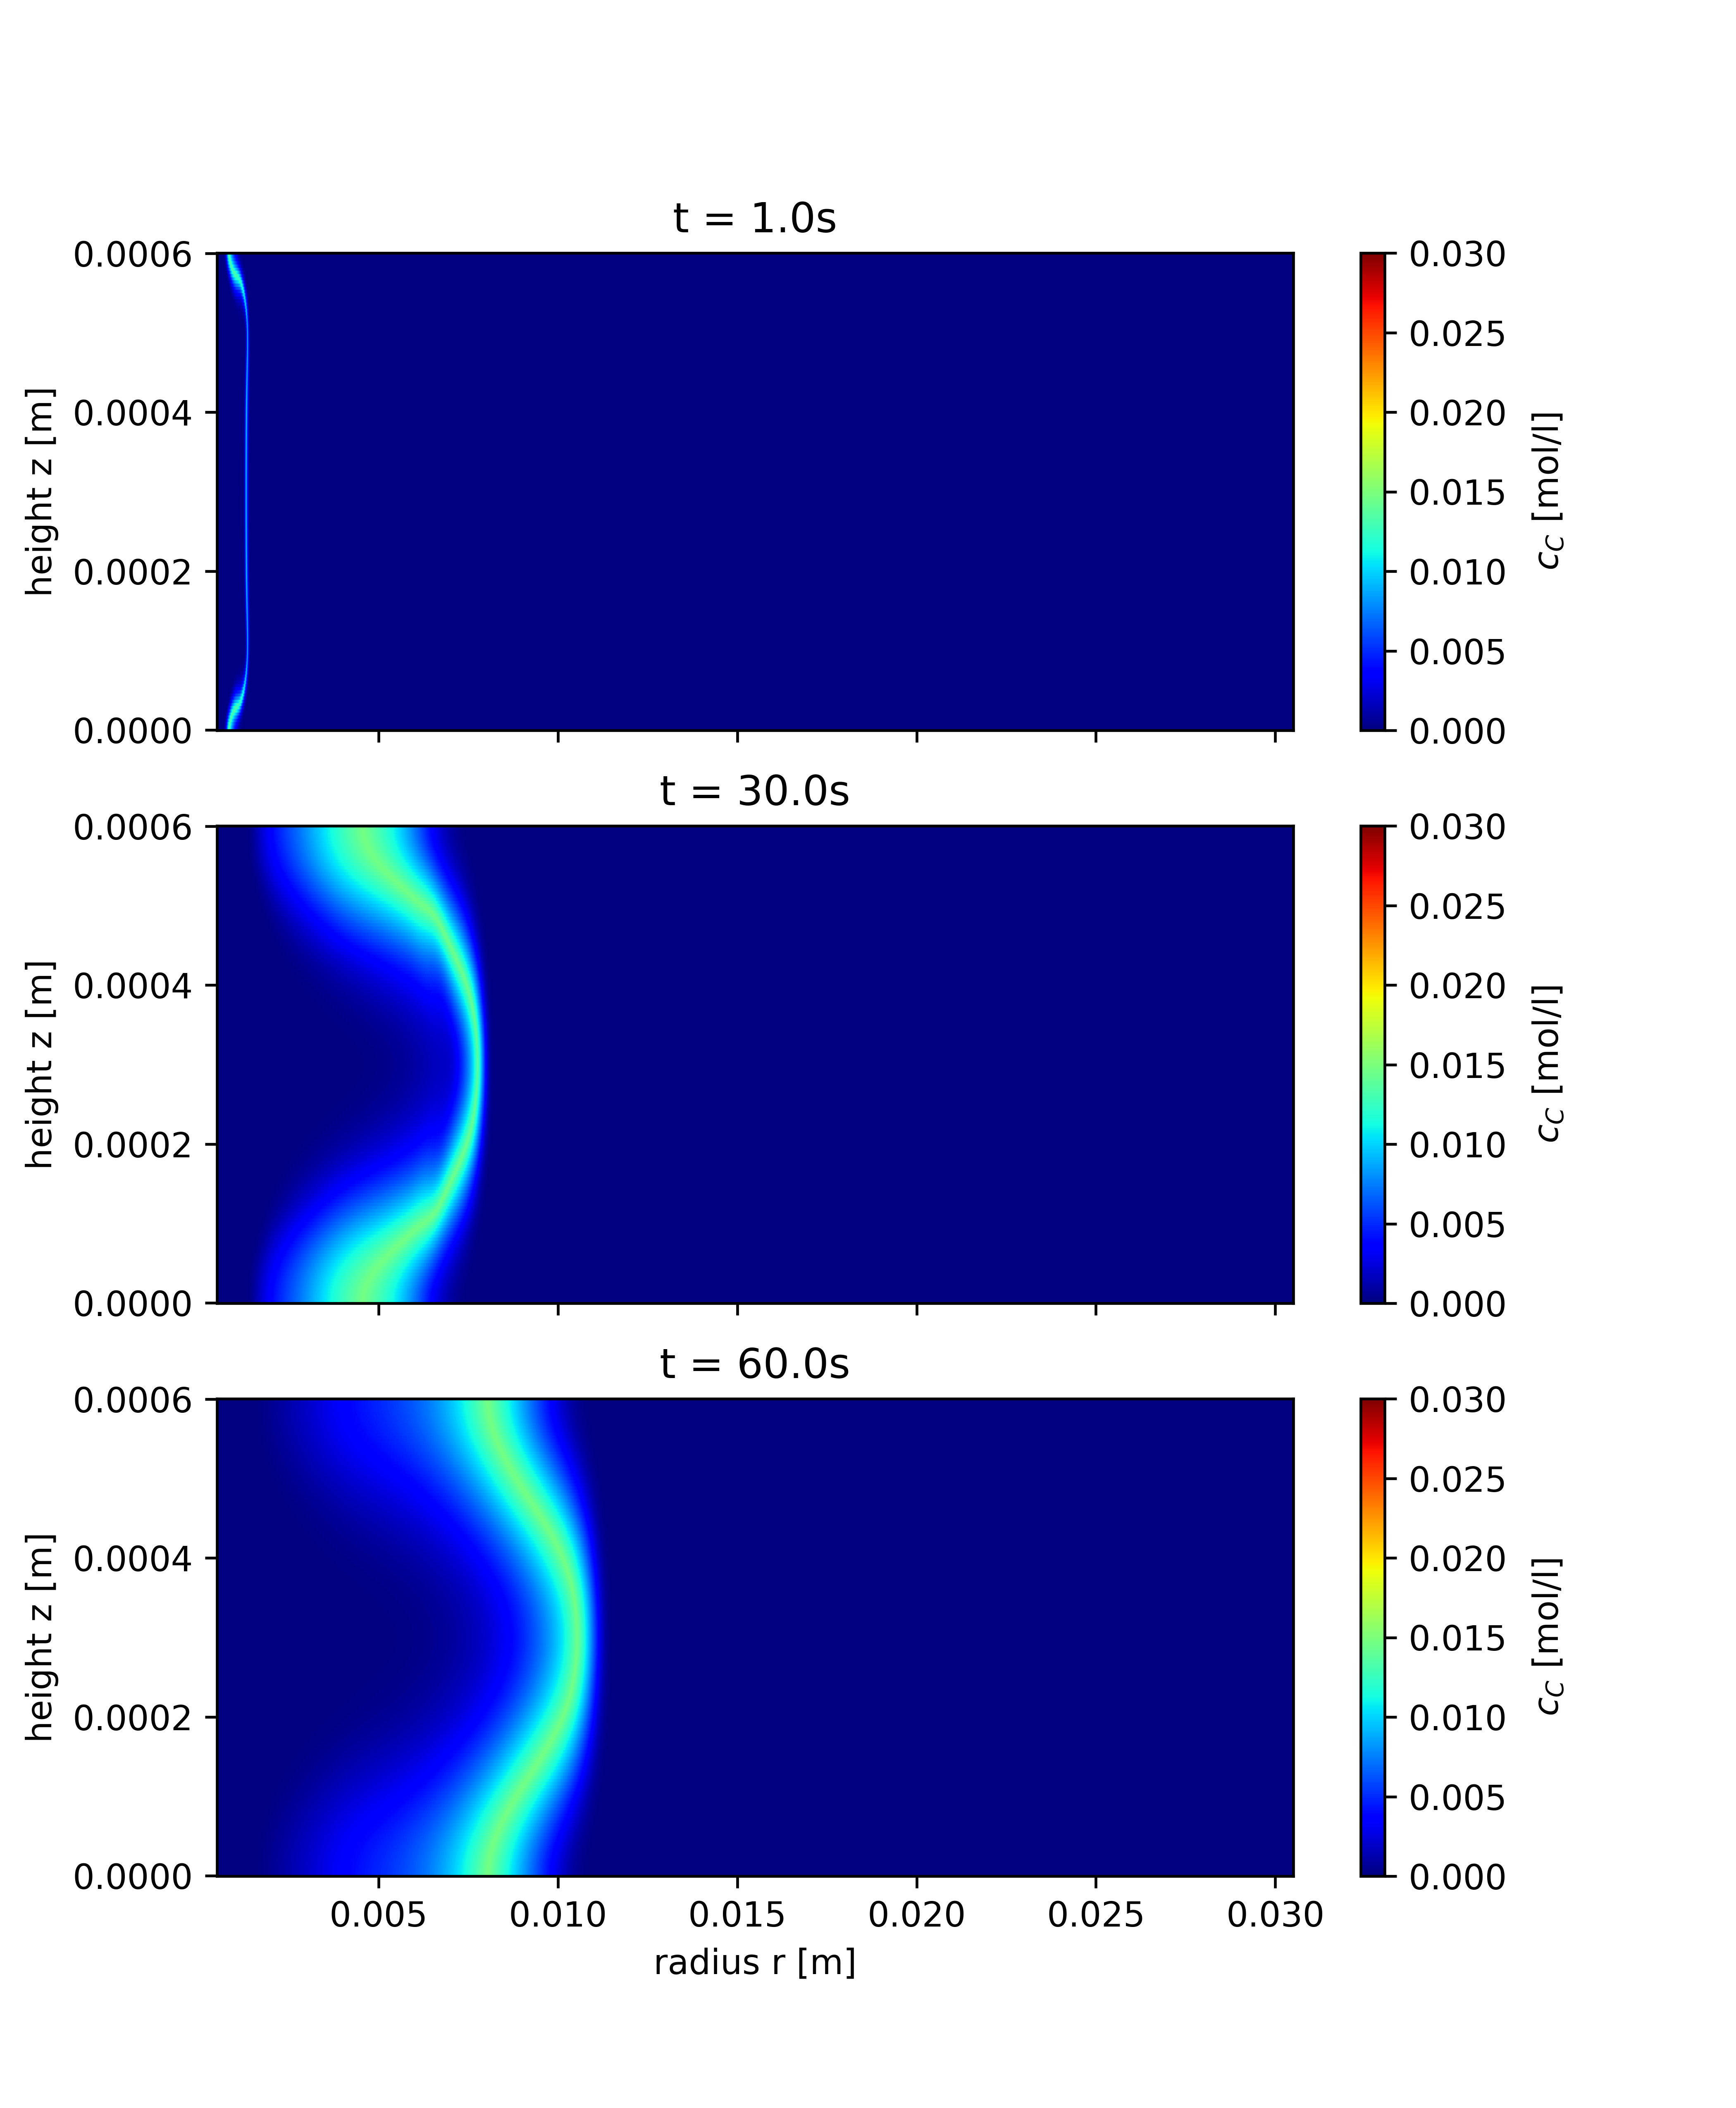
\includegraphics[angle=0, scale=0.41]{front_shape1} }}%
	\qquad
	\subfloat[\centering front shape for h0.2mm Pe2050 Sc2430]{{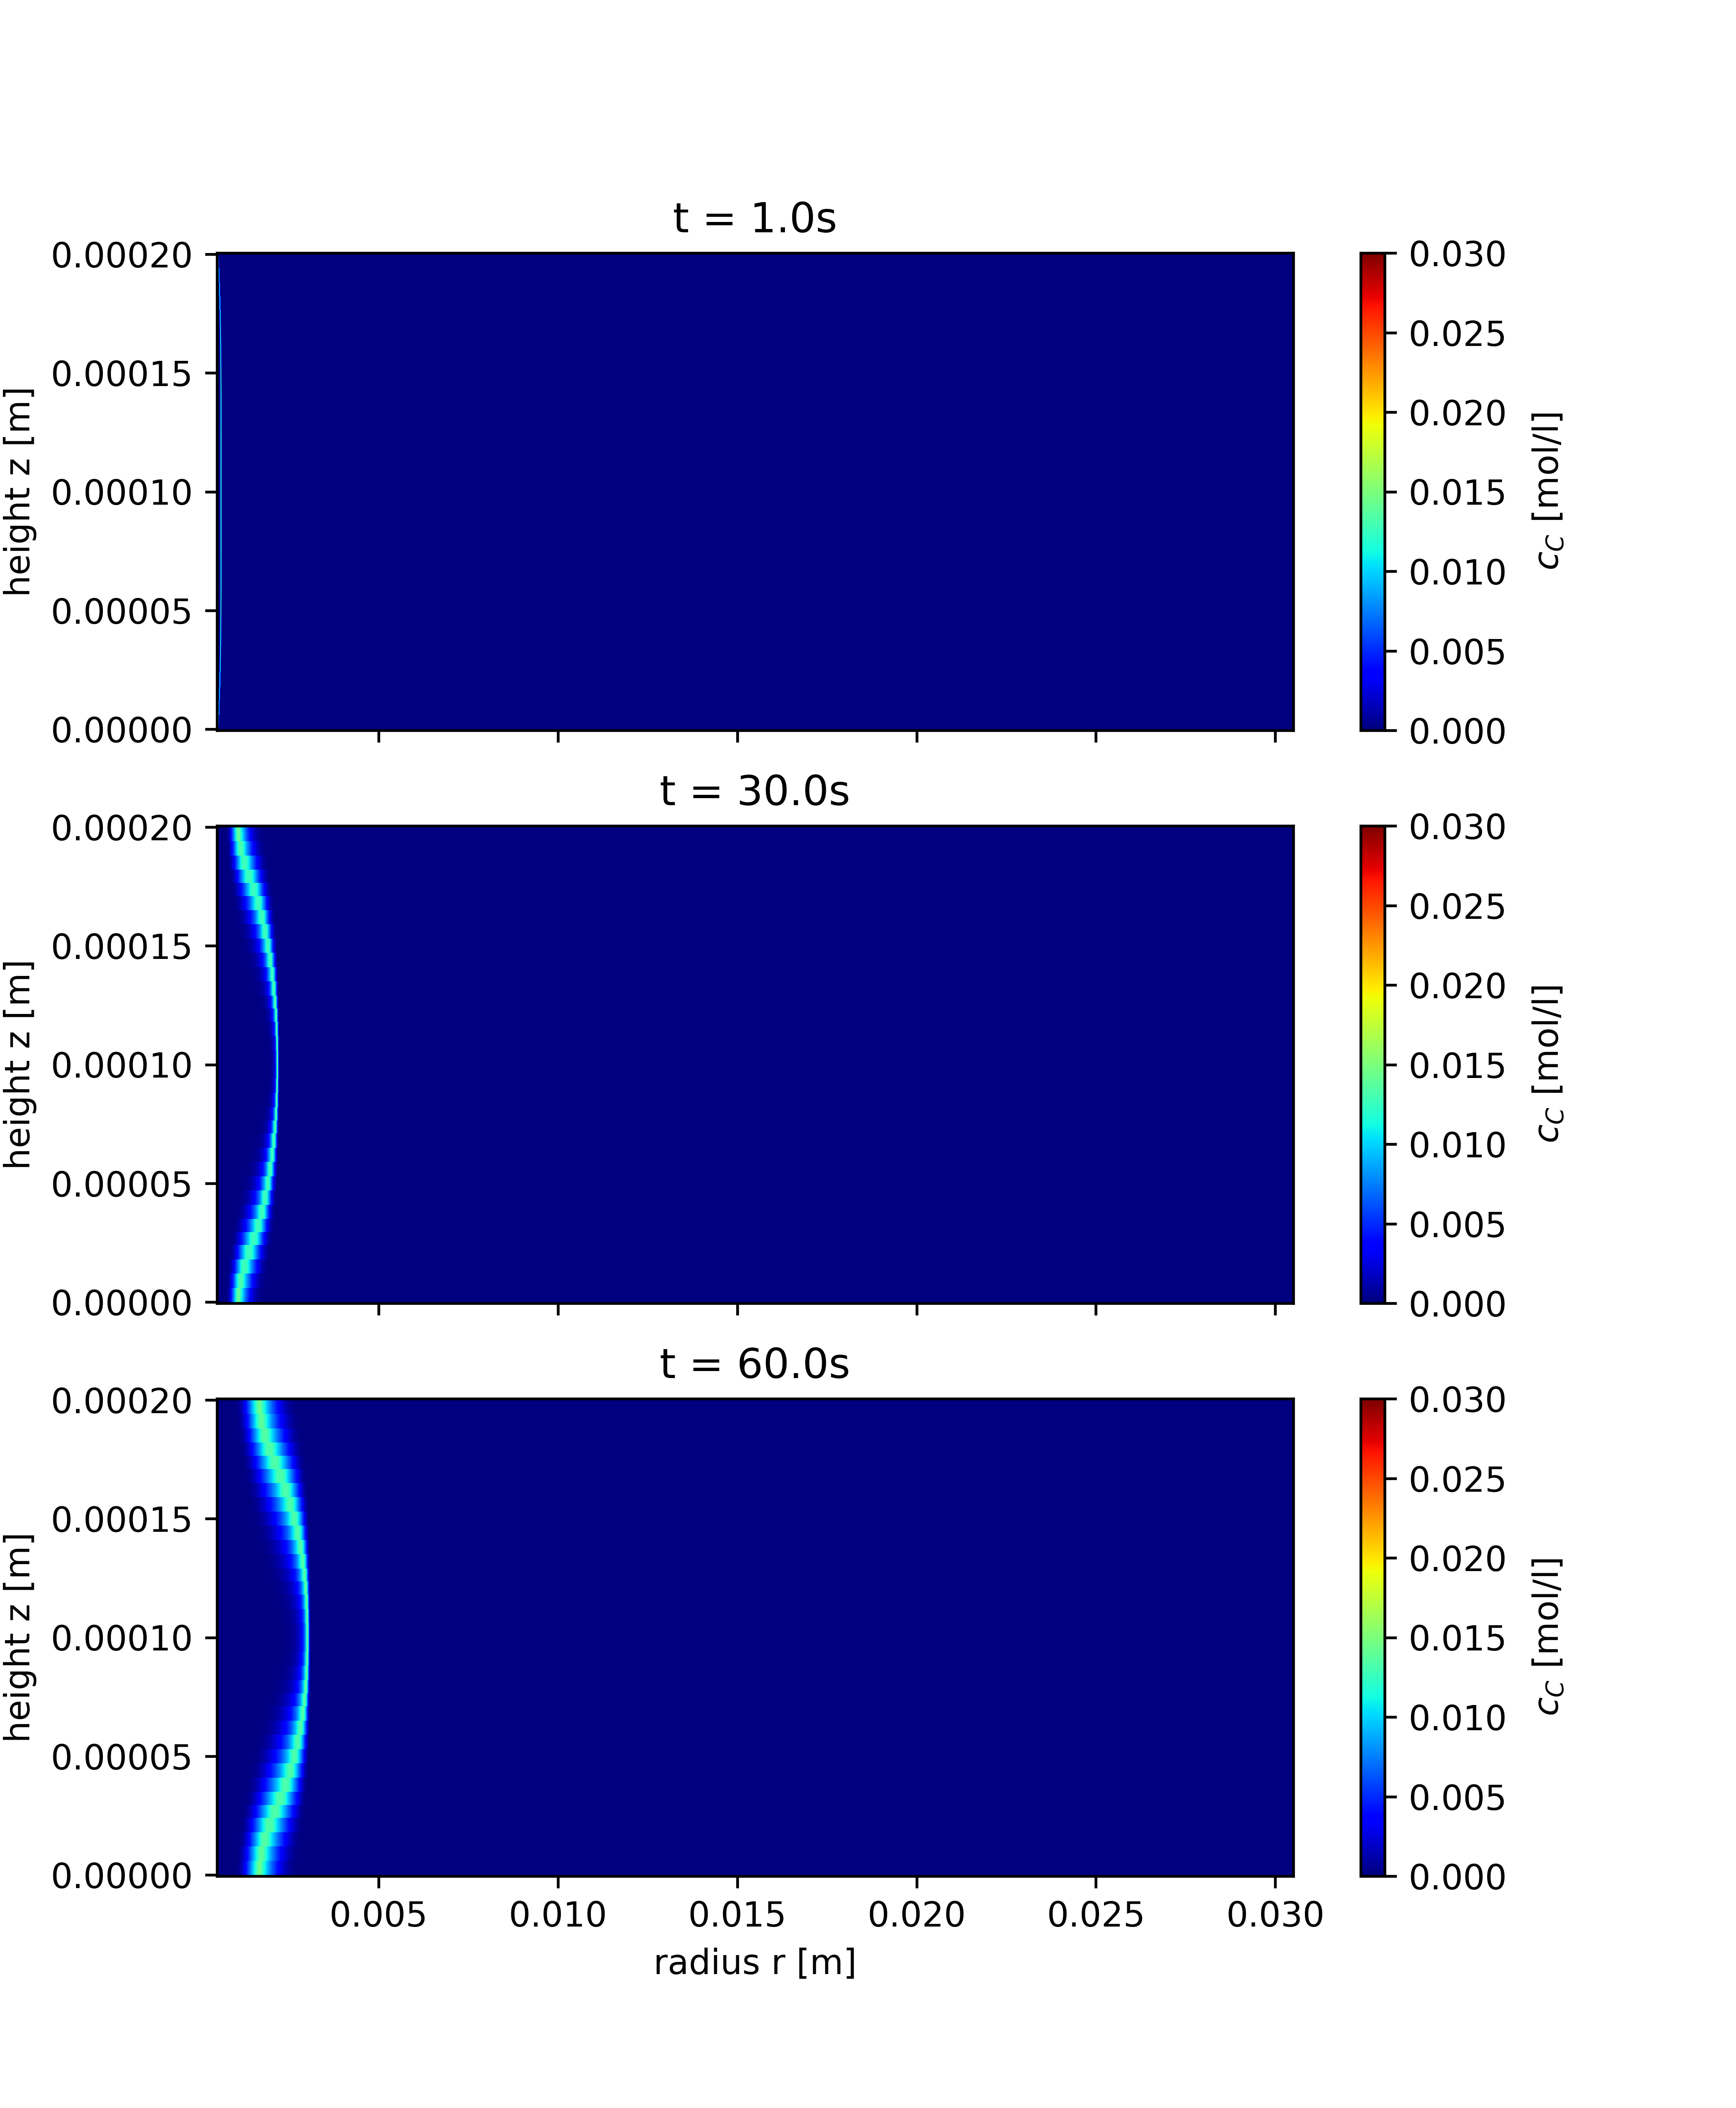
\includegraphics[angle=0, scale=0.41]{front_shape2} }}%
	\caption{example front shapes}%
	\label{fig: shape_examp}%
\end{figure}

\section{front positions}

The front positions behave in a similar way for all 3 reactor geometries. So in \autoref{fig: front_pos_h2_SC12E4} and \autoref{fig: front_pos_h2_SC243E3} the positions for both Schmidt-Number are shown for the geometry containing a gap height of 0.2mm.
% two figures on same page
\begin{figure}[htbp]
	\centering
	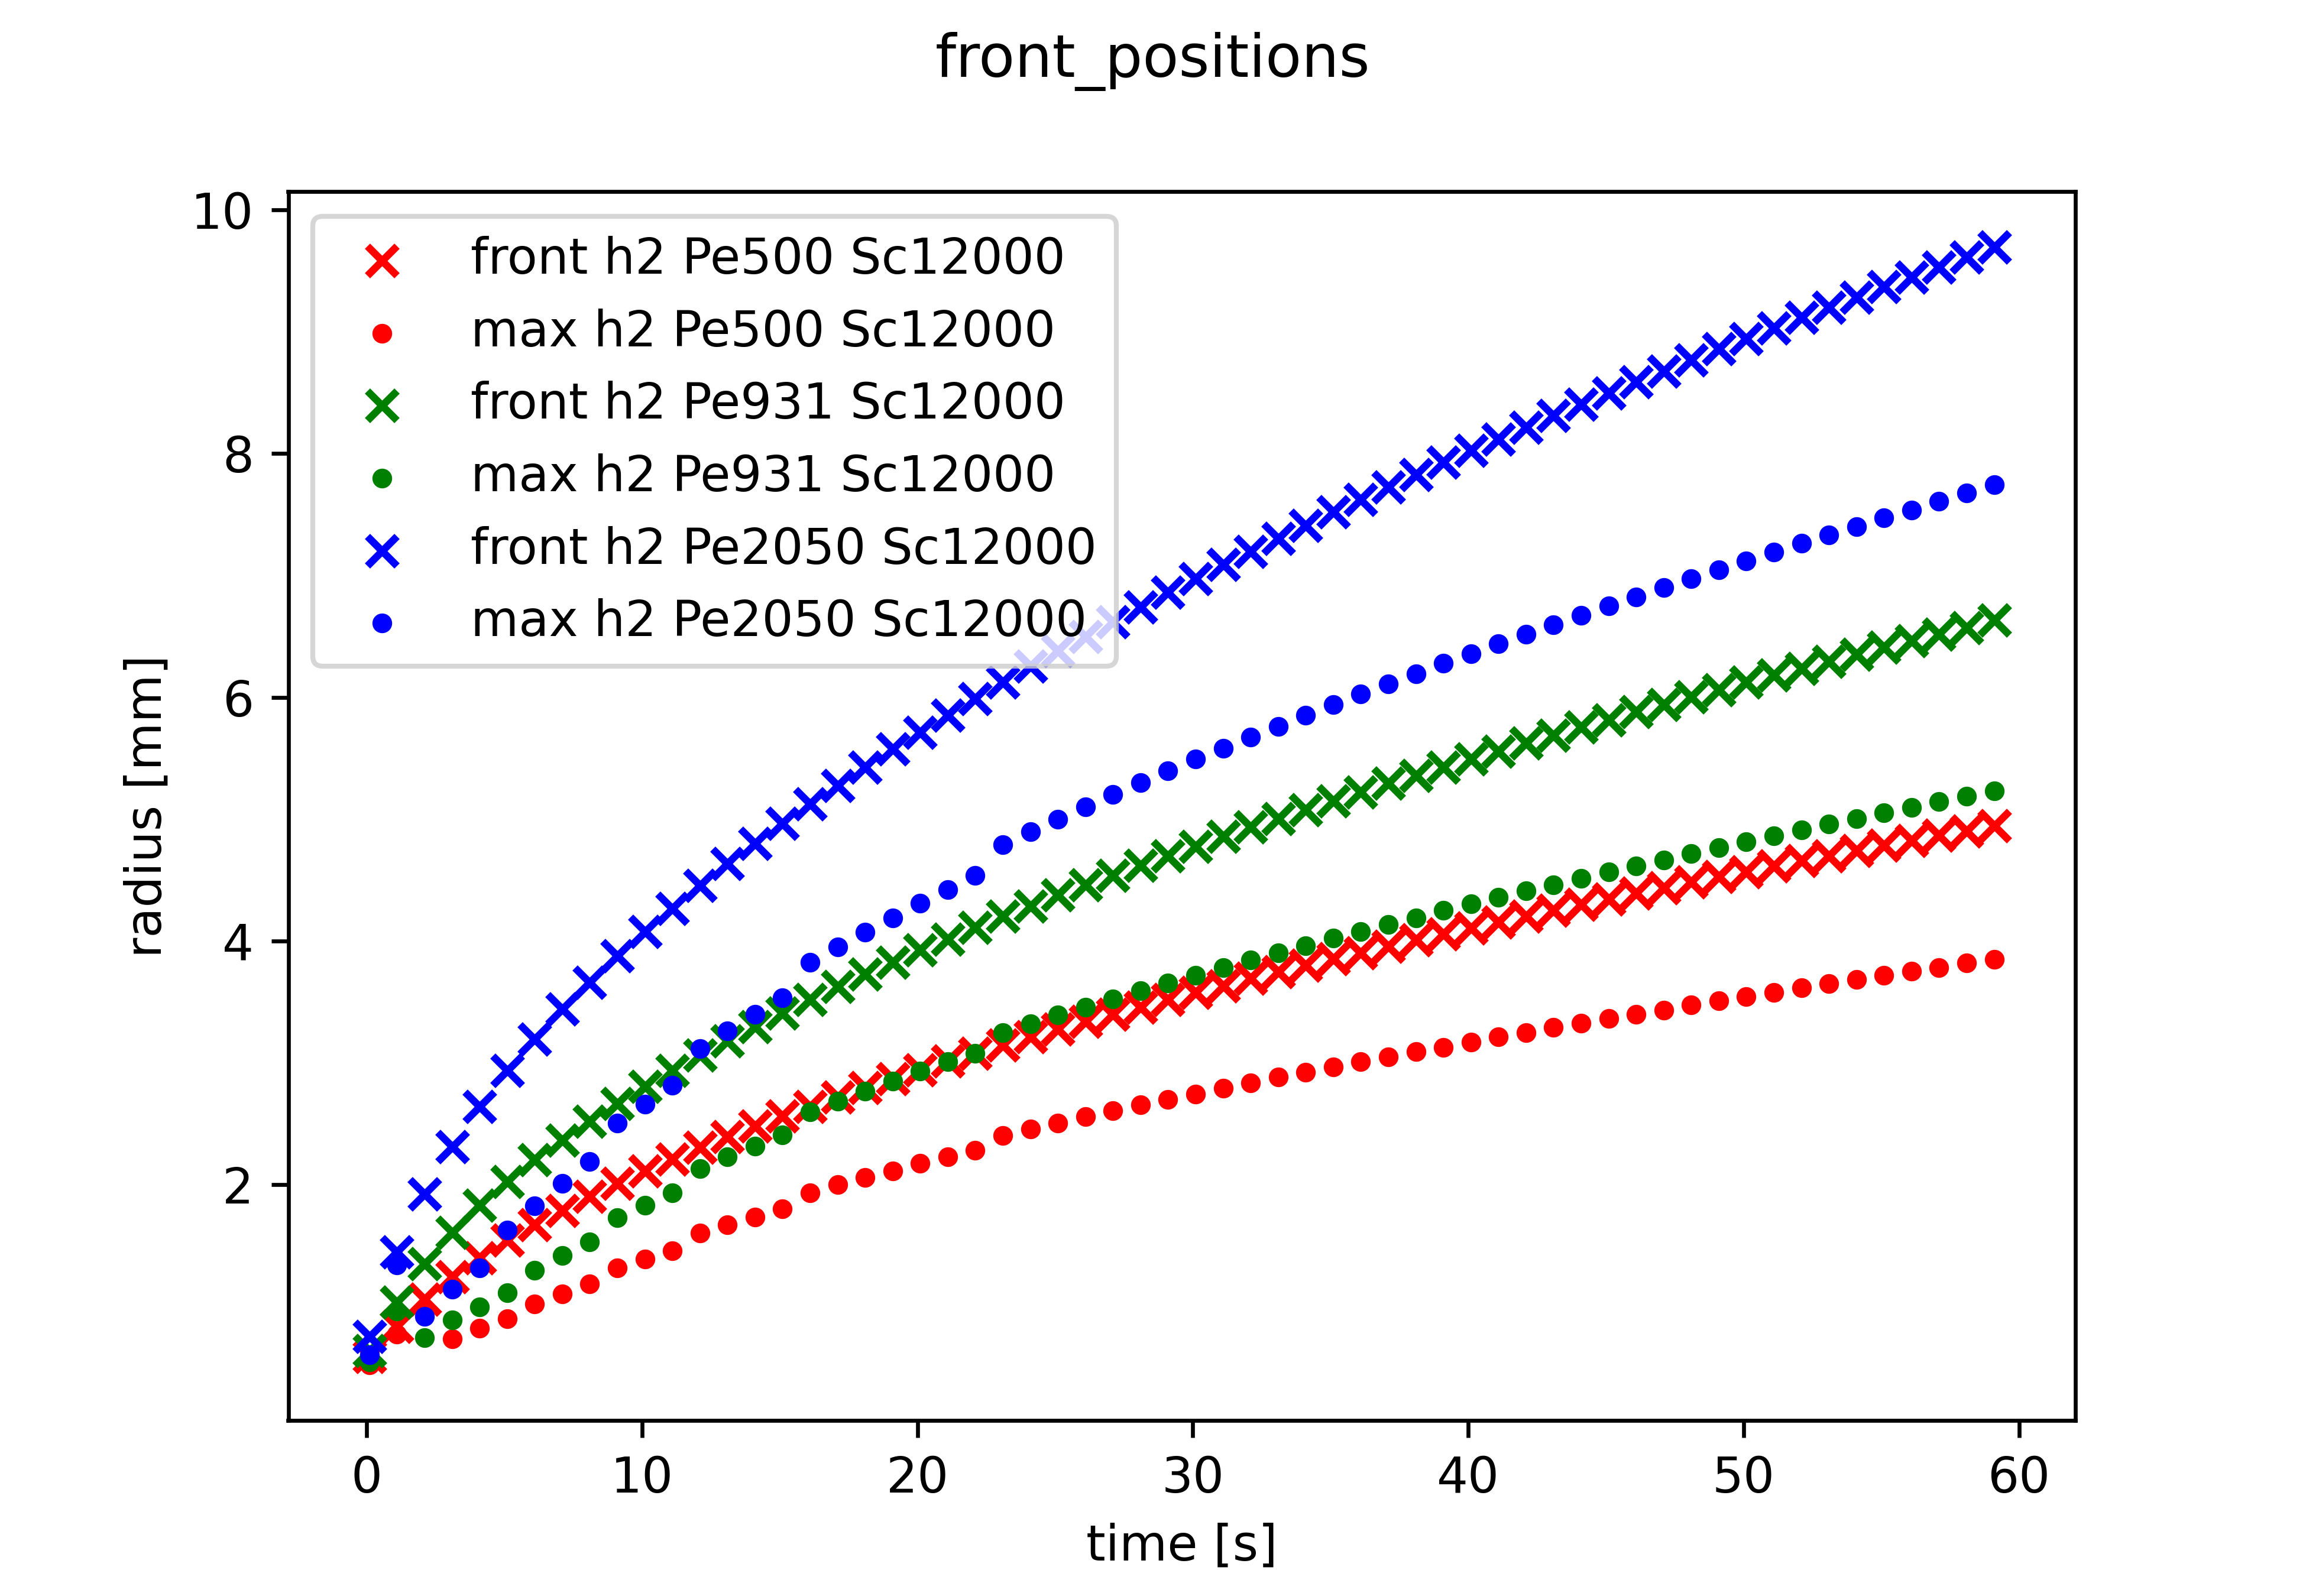
\includegraphics[width=.9\linewidth]{front_pos_h2_SC12E4}
	\caption{front positions for h 0.2mm Sc 12000\label{fig: front_pos_h2_SC12E4}}\bigskip
	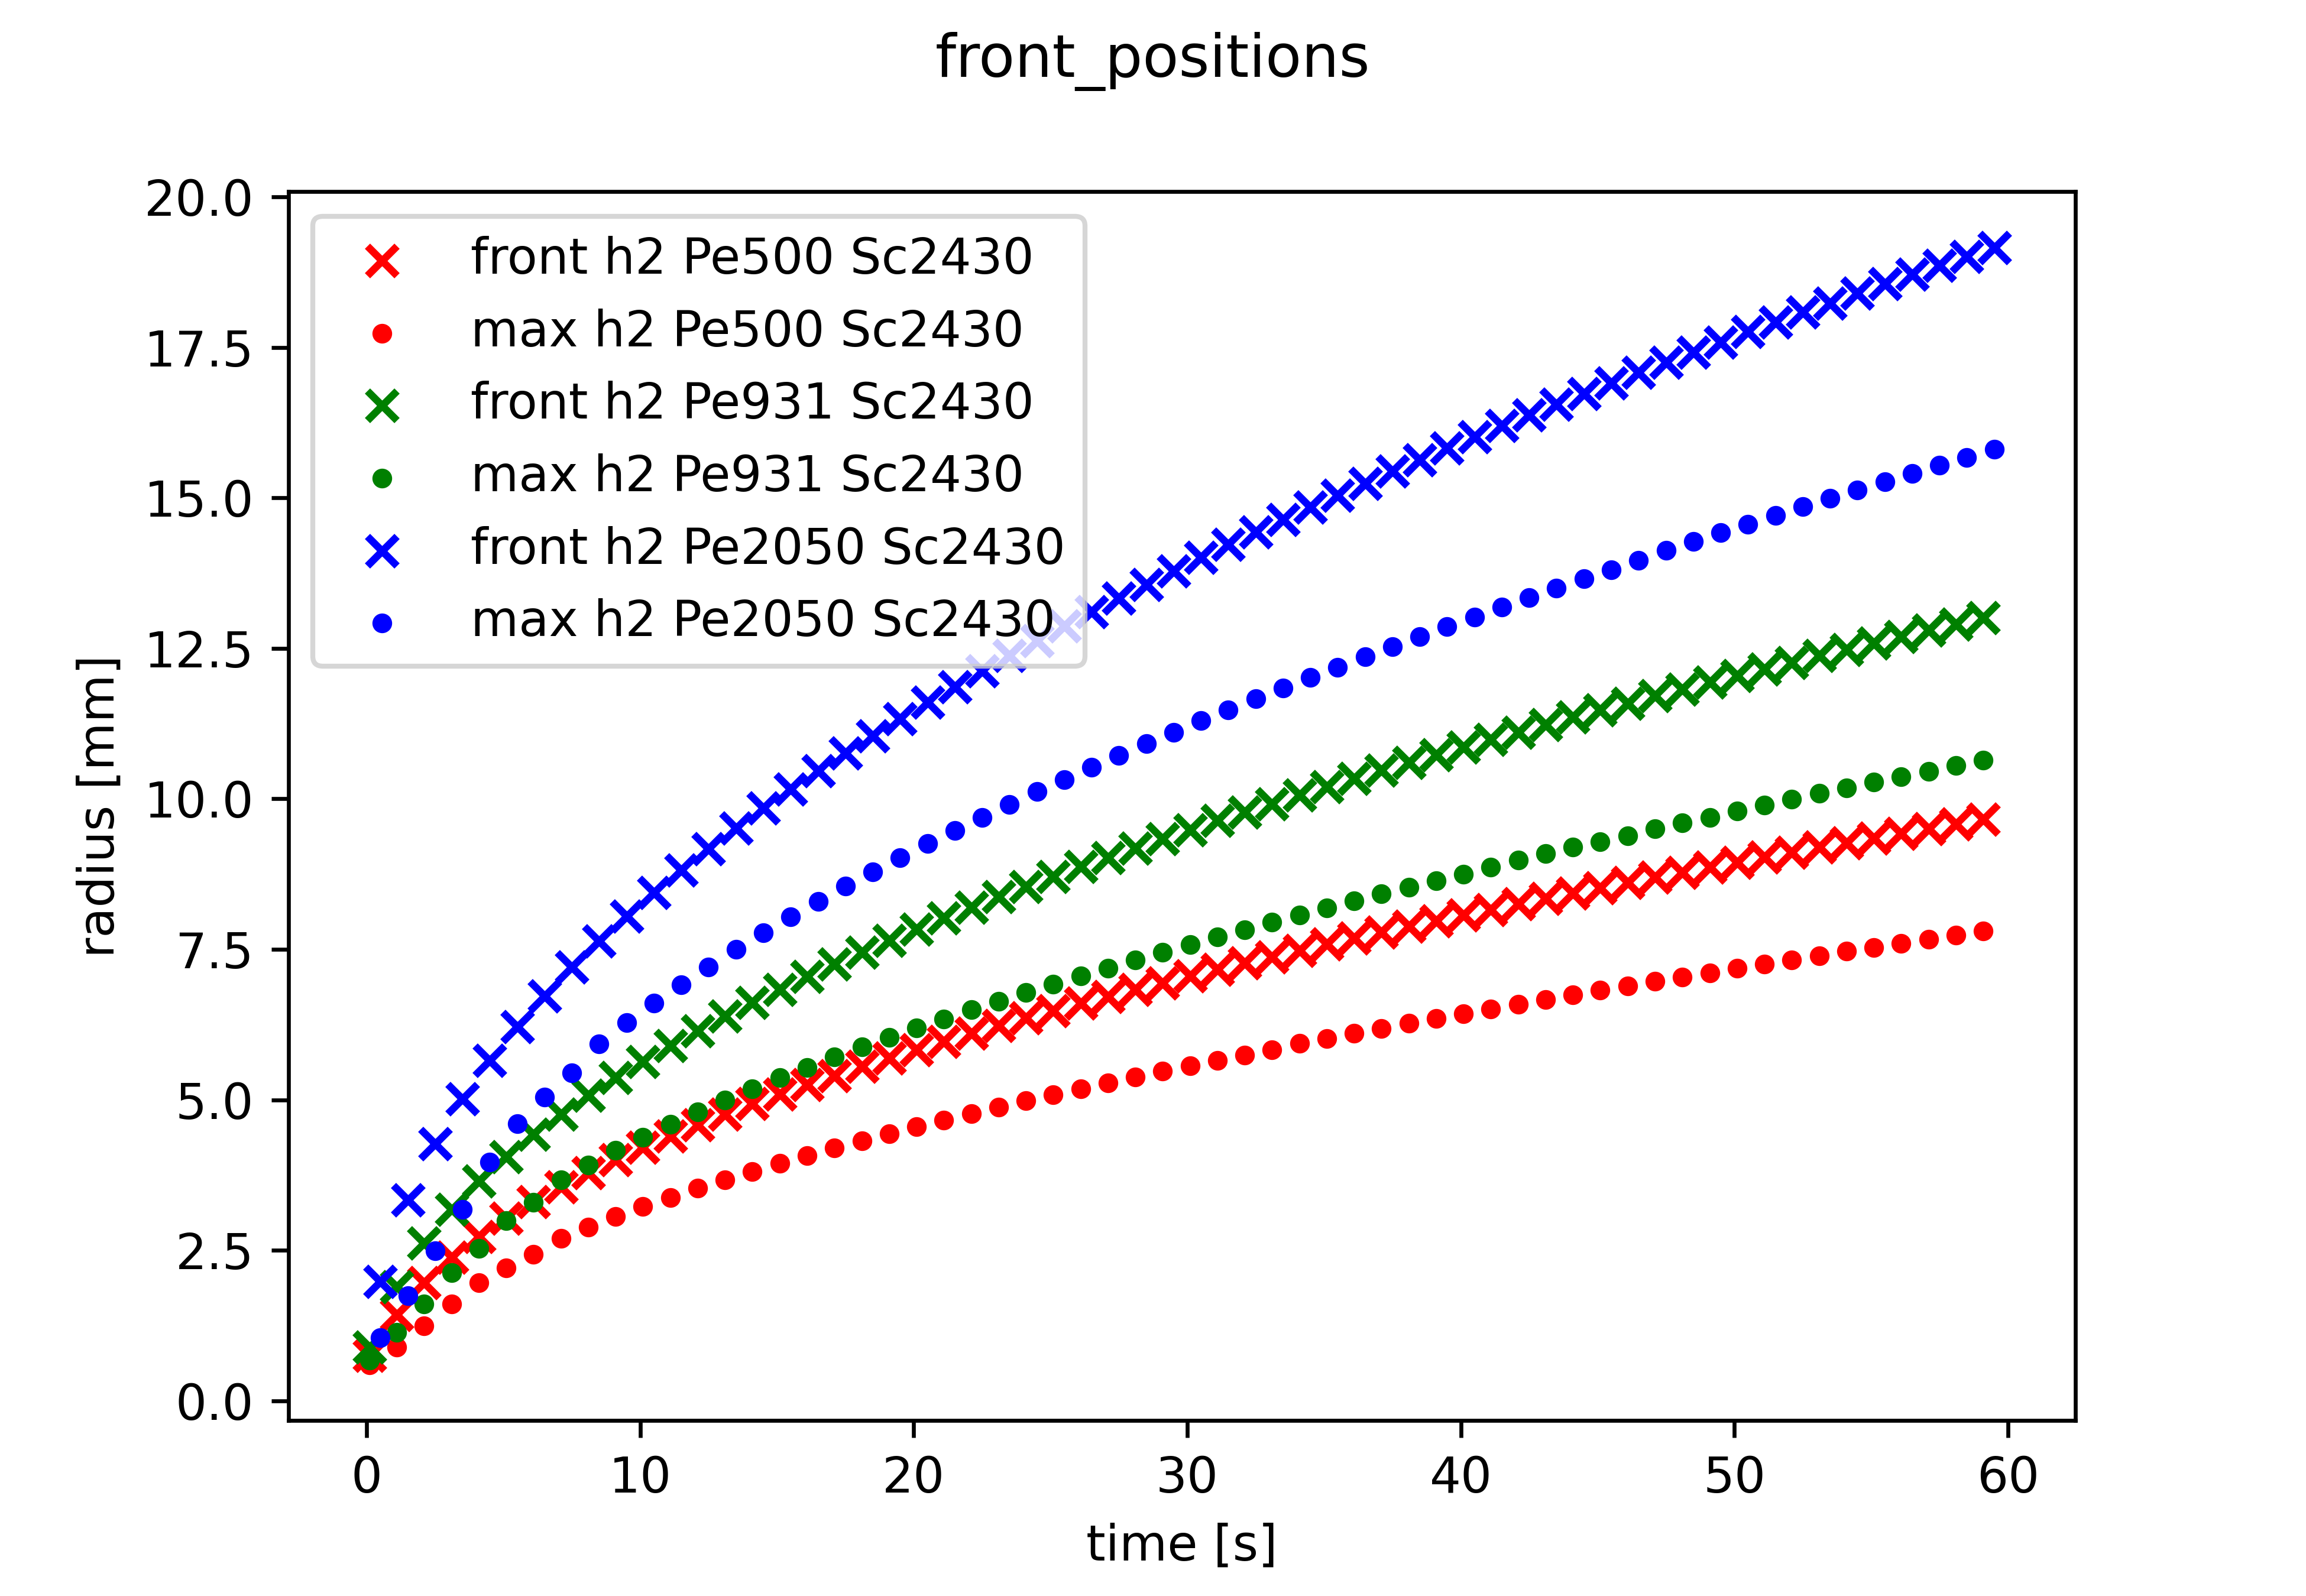
\includegraphics[width=.9\linewidth]{front_pos_h2_SC243E3}
	\caption{front positions for h 0.2mm Sc 2430\label{fig: front_pos_h2_SC243E3}}
\end{figure}

From these two graphs it can be seen that the front positions travel speed decays over time, following a behaviour close to a  square root function. The front and maximum travel faster for higher Peclet-Numbers, which can be explained by the different input velocities. The maxima positions show a similar behaviour to the front positions. 
With decreasing input velocity the difference between the fronts front and maximum positions decreases. The decrease is more significant for cases with lower Peclet-Numbers. For these cases, due to their lower inlet velocity, the distance between the front and maximum is lower. An increase in distance can be seen when comparing plots for Pecelt-Numbers of 931 with 2430.

When comparing the plots for Schmidt-Number 2430 with the one for a Schmidt-Number of 12000 it can be observed that all fronts travel nearly double the distance within the same time of 60 seconds. This can be explained mainly by the lower diffusion coefficient for the higher Schmidt-Number case. The diffusion coefficient for the lower Schmidt-Number case is $4 \text{.}11 \cdot 10^{-10} \left[ \frac{\mathrm{m^2}}{\mathrm{s}} \right]$ and the one for the higher case is $1\text{.}0 \cdot 10^{-10} \left[ \frac{\mathrm{m^2}}{\mathrm{s}} \right]$.
Since the velocity magnitude decreases very quickly for a axisymmetric reactor (see \autoref{fig: field_example}) diffusion plays a more and more significant role while the front travels through the reactor. So the diffusive fraction taking part in the front's forward travel is getting higher the further the front gets away from the inlet. The diffusion coefficient has an influence on the fronts width as well which will be look at within the following section.

\section{front widths}

The fronts widths behaviour is quite different for each reactor geometry so each one will be looked at starting with the smallest gap height of 0.2mm.  

\begin{figure}[htbp]
	\centering
	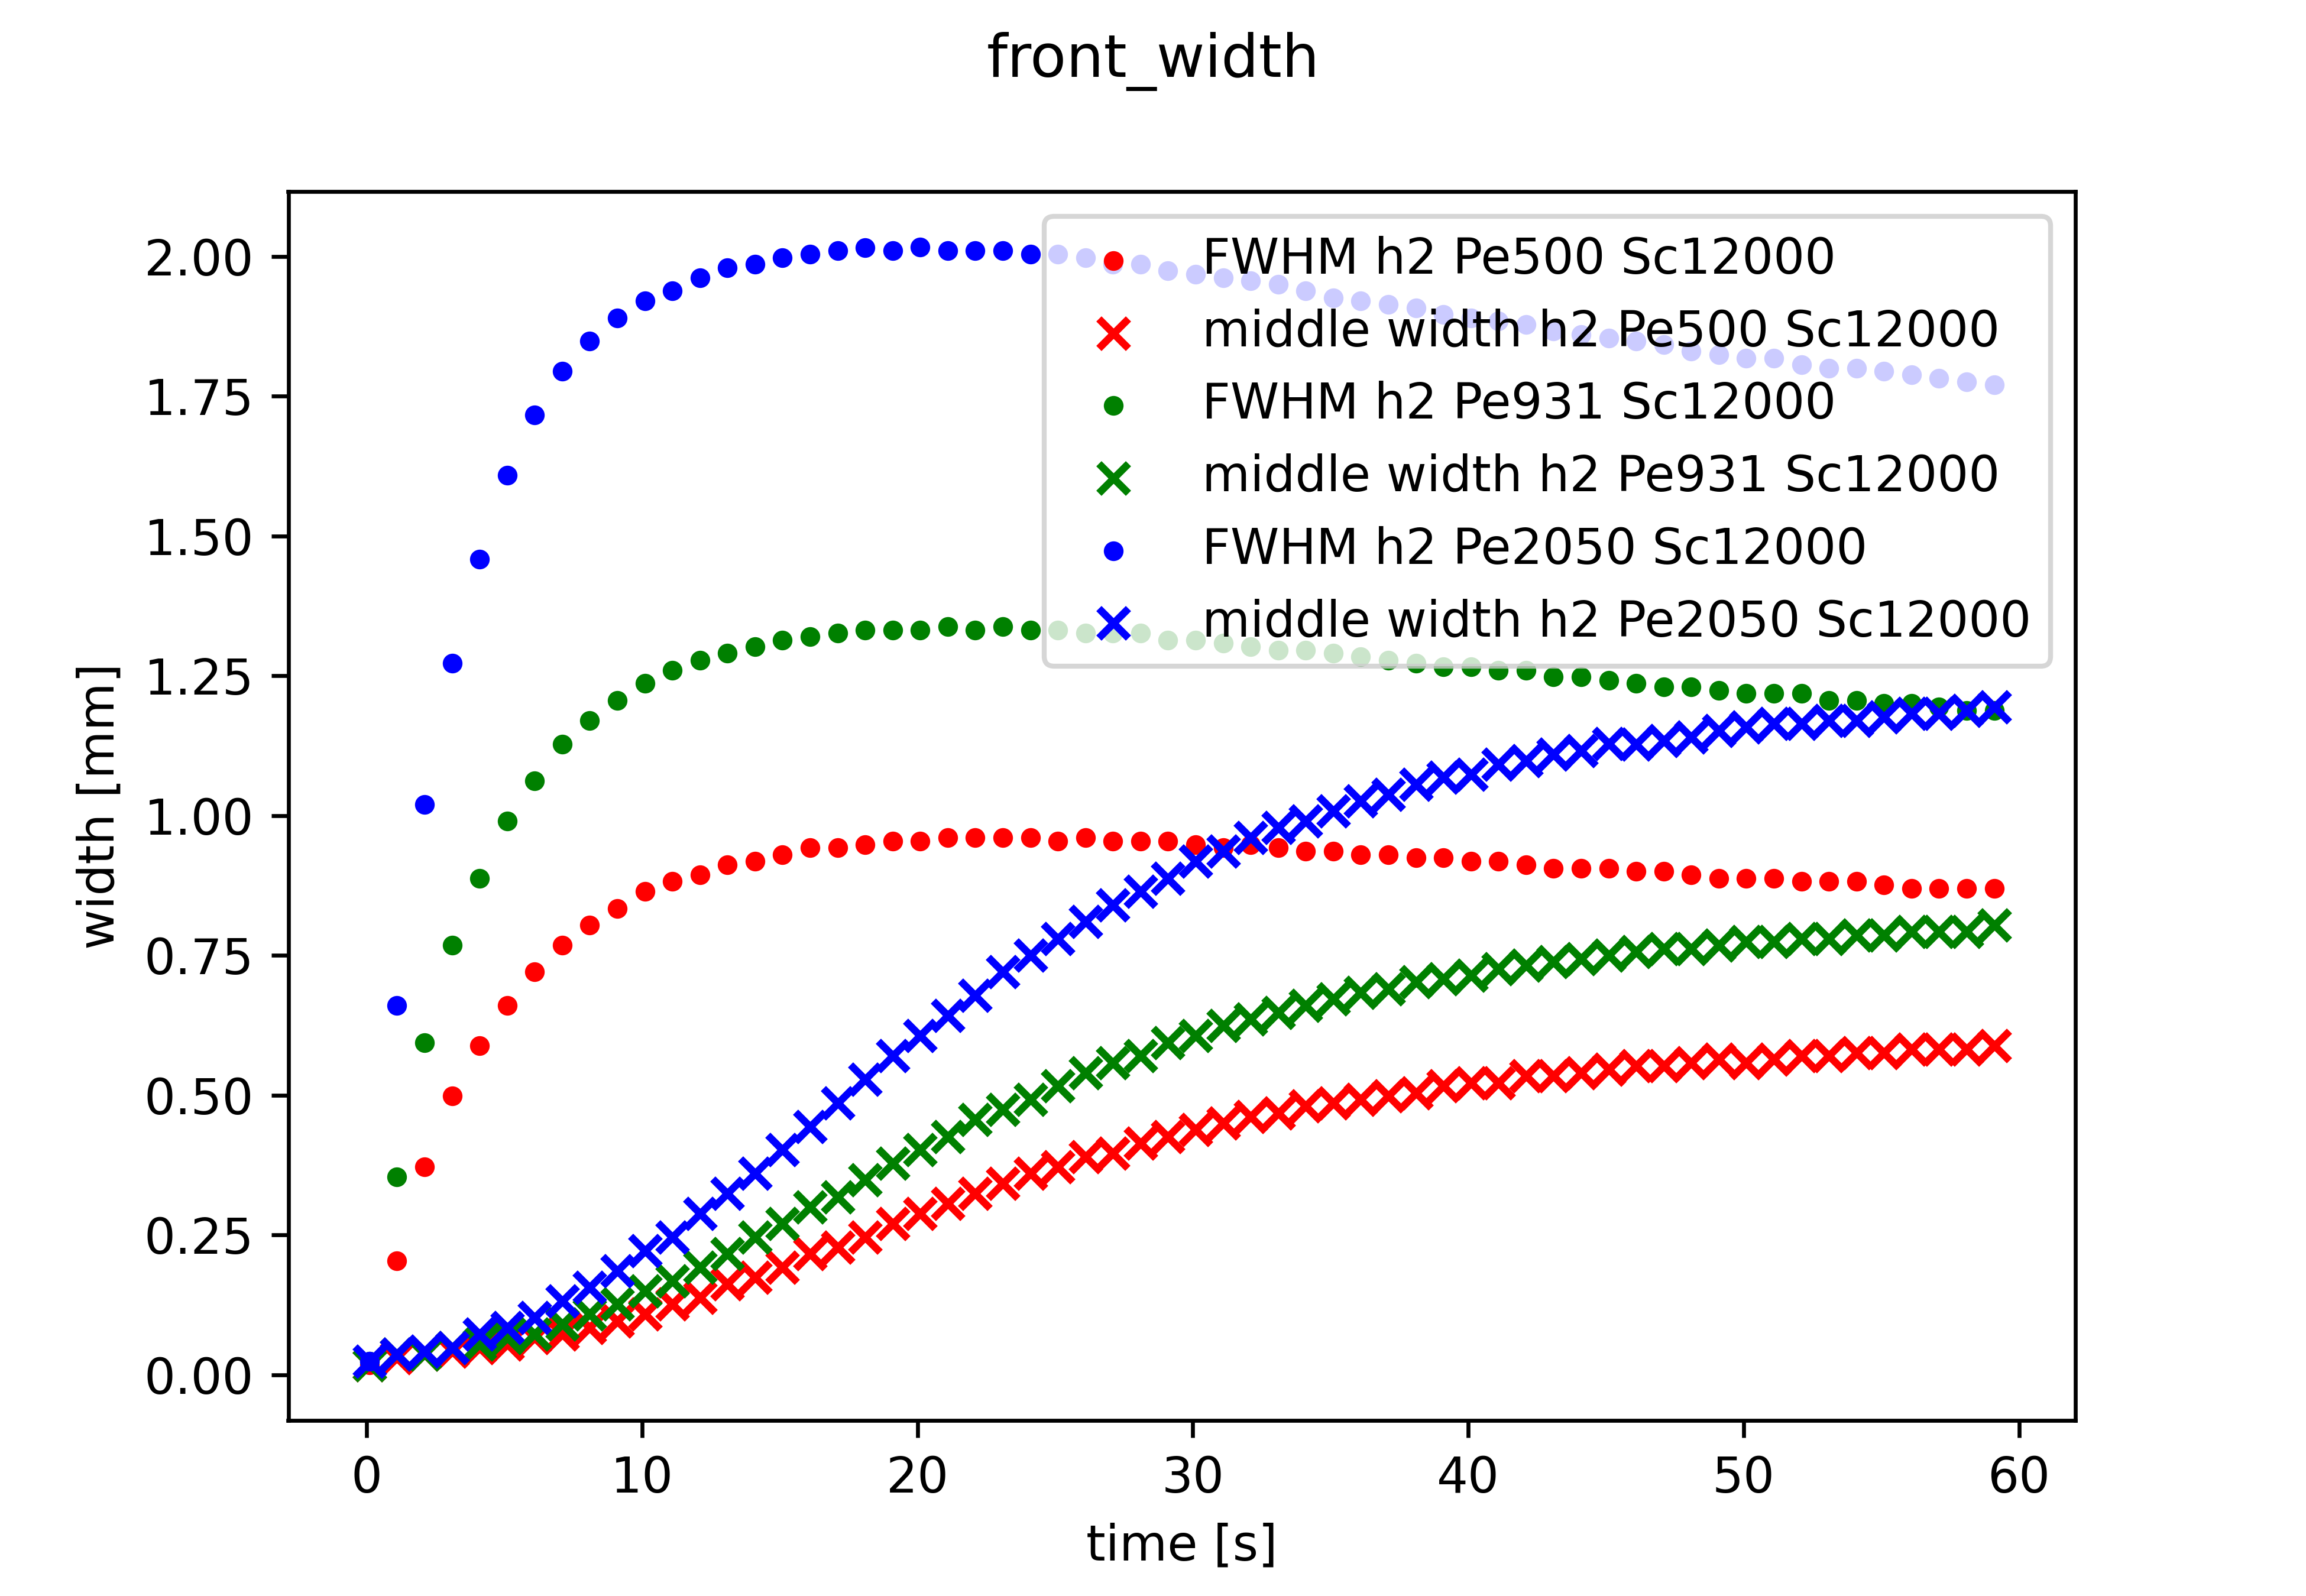
\includegraphics[width=.9\linewidth]{front_width_h2_SC12E4}
	\caption{front widths for h 0.2mm Sc 12000\label{fig: front_width_h2_SC12E4}}\bigskip
	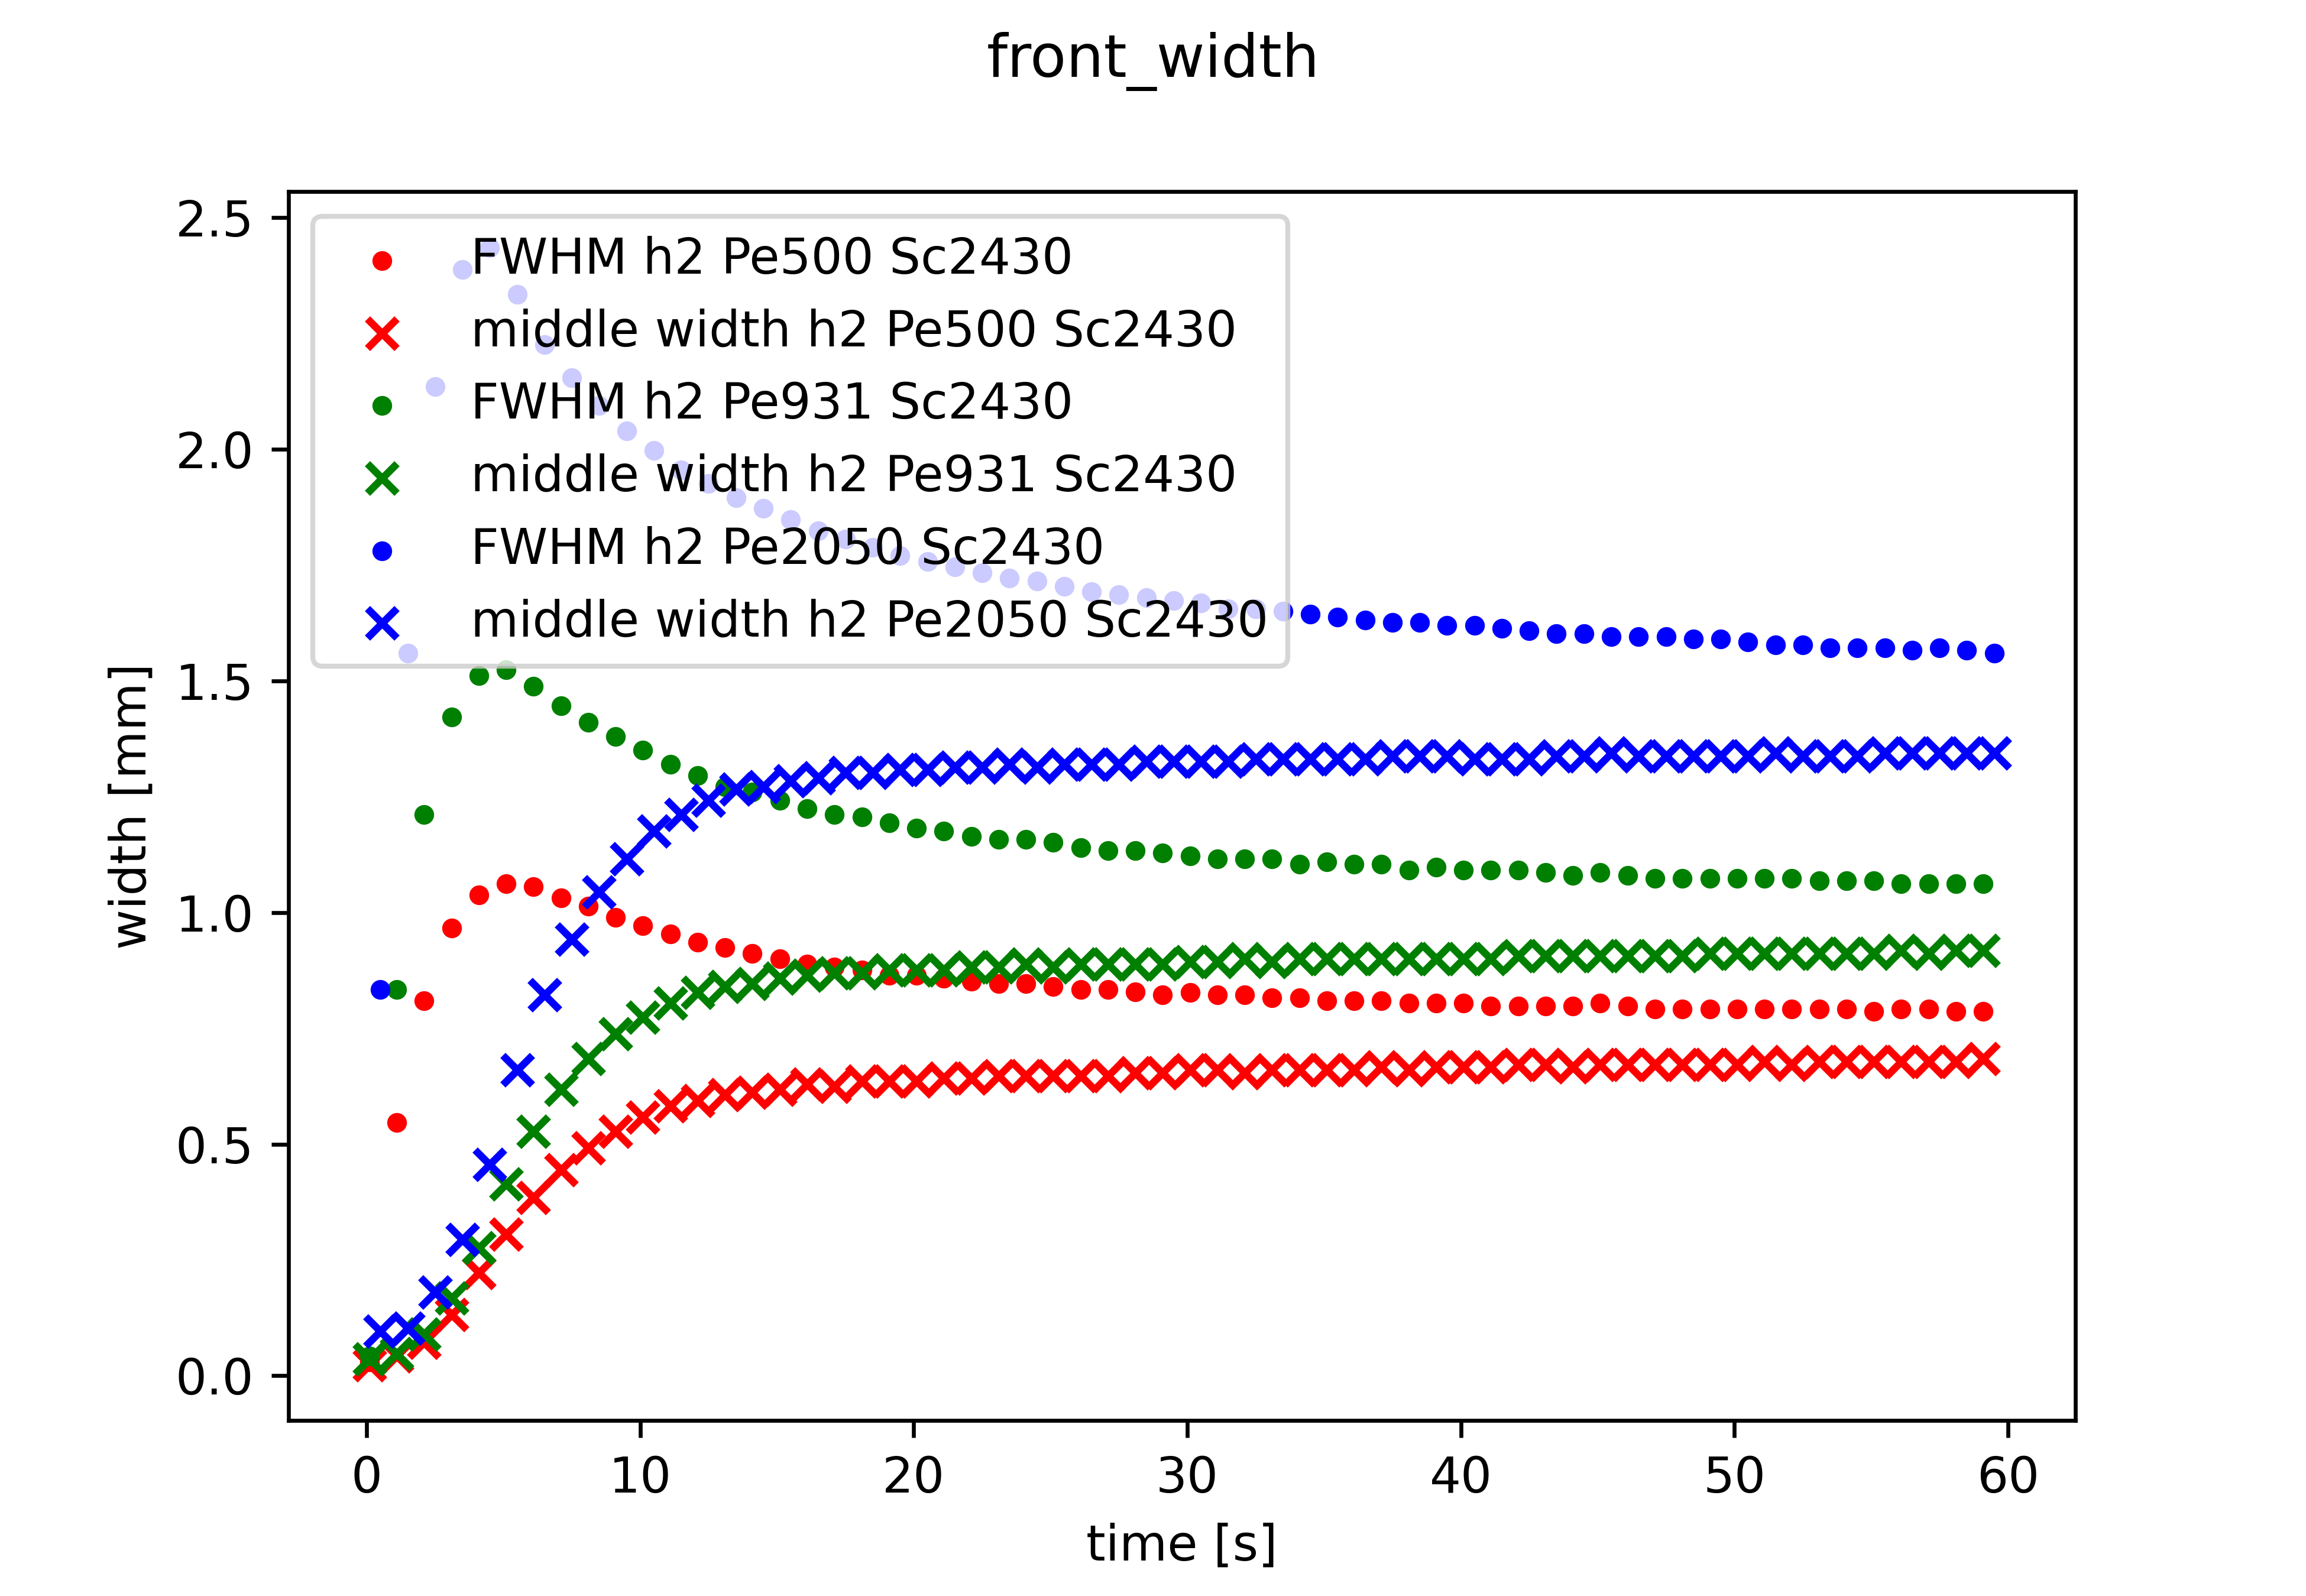
\includegraphics[width=.9\linewidth]{front_width_h2_SC243E3}
	\caption{front widths for h 0.2mm Sc 2430\label{fig: front_width_pos_h2_SC243E3}}
\end{figure}

\begin{figure}[htbp]
	\centering
	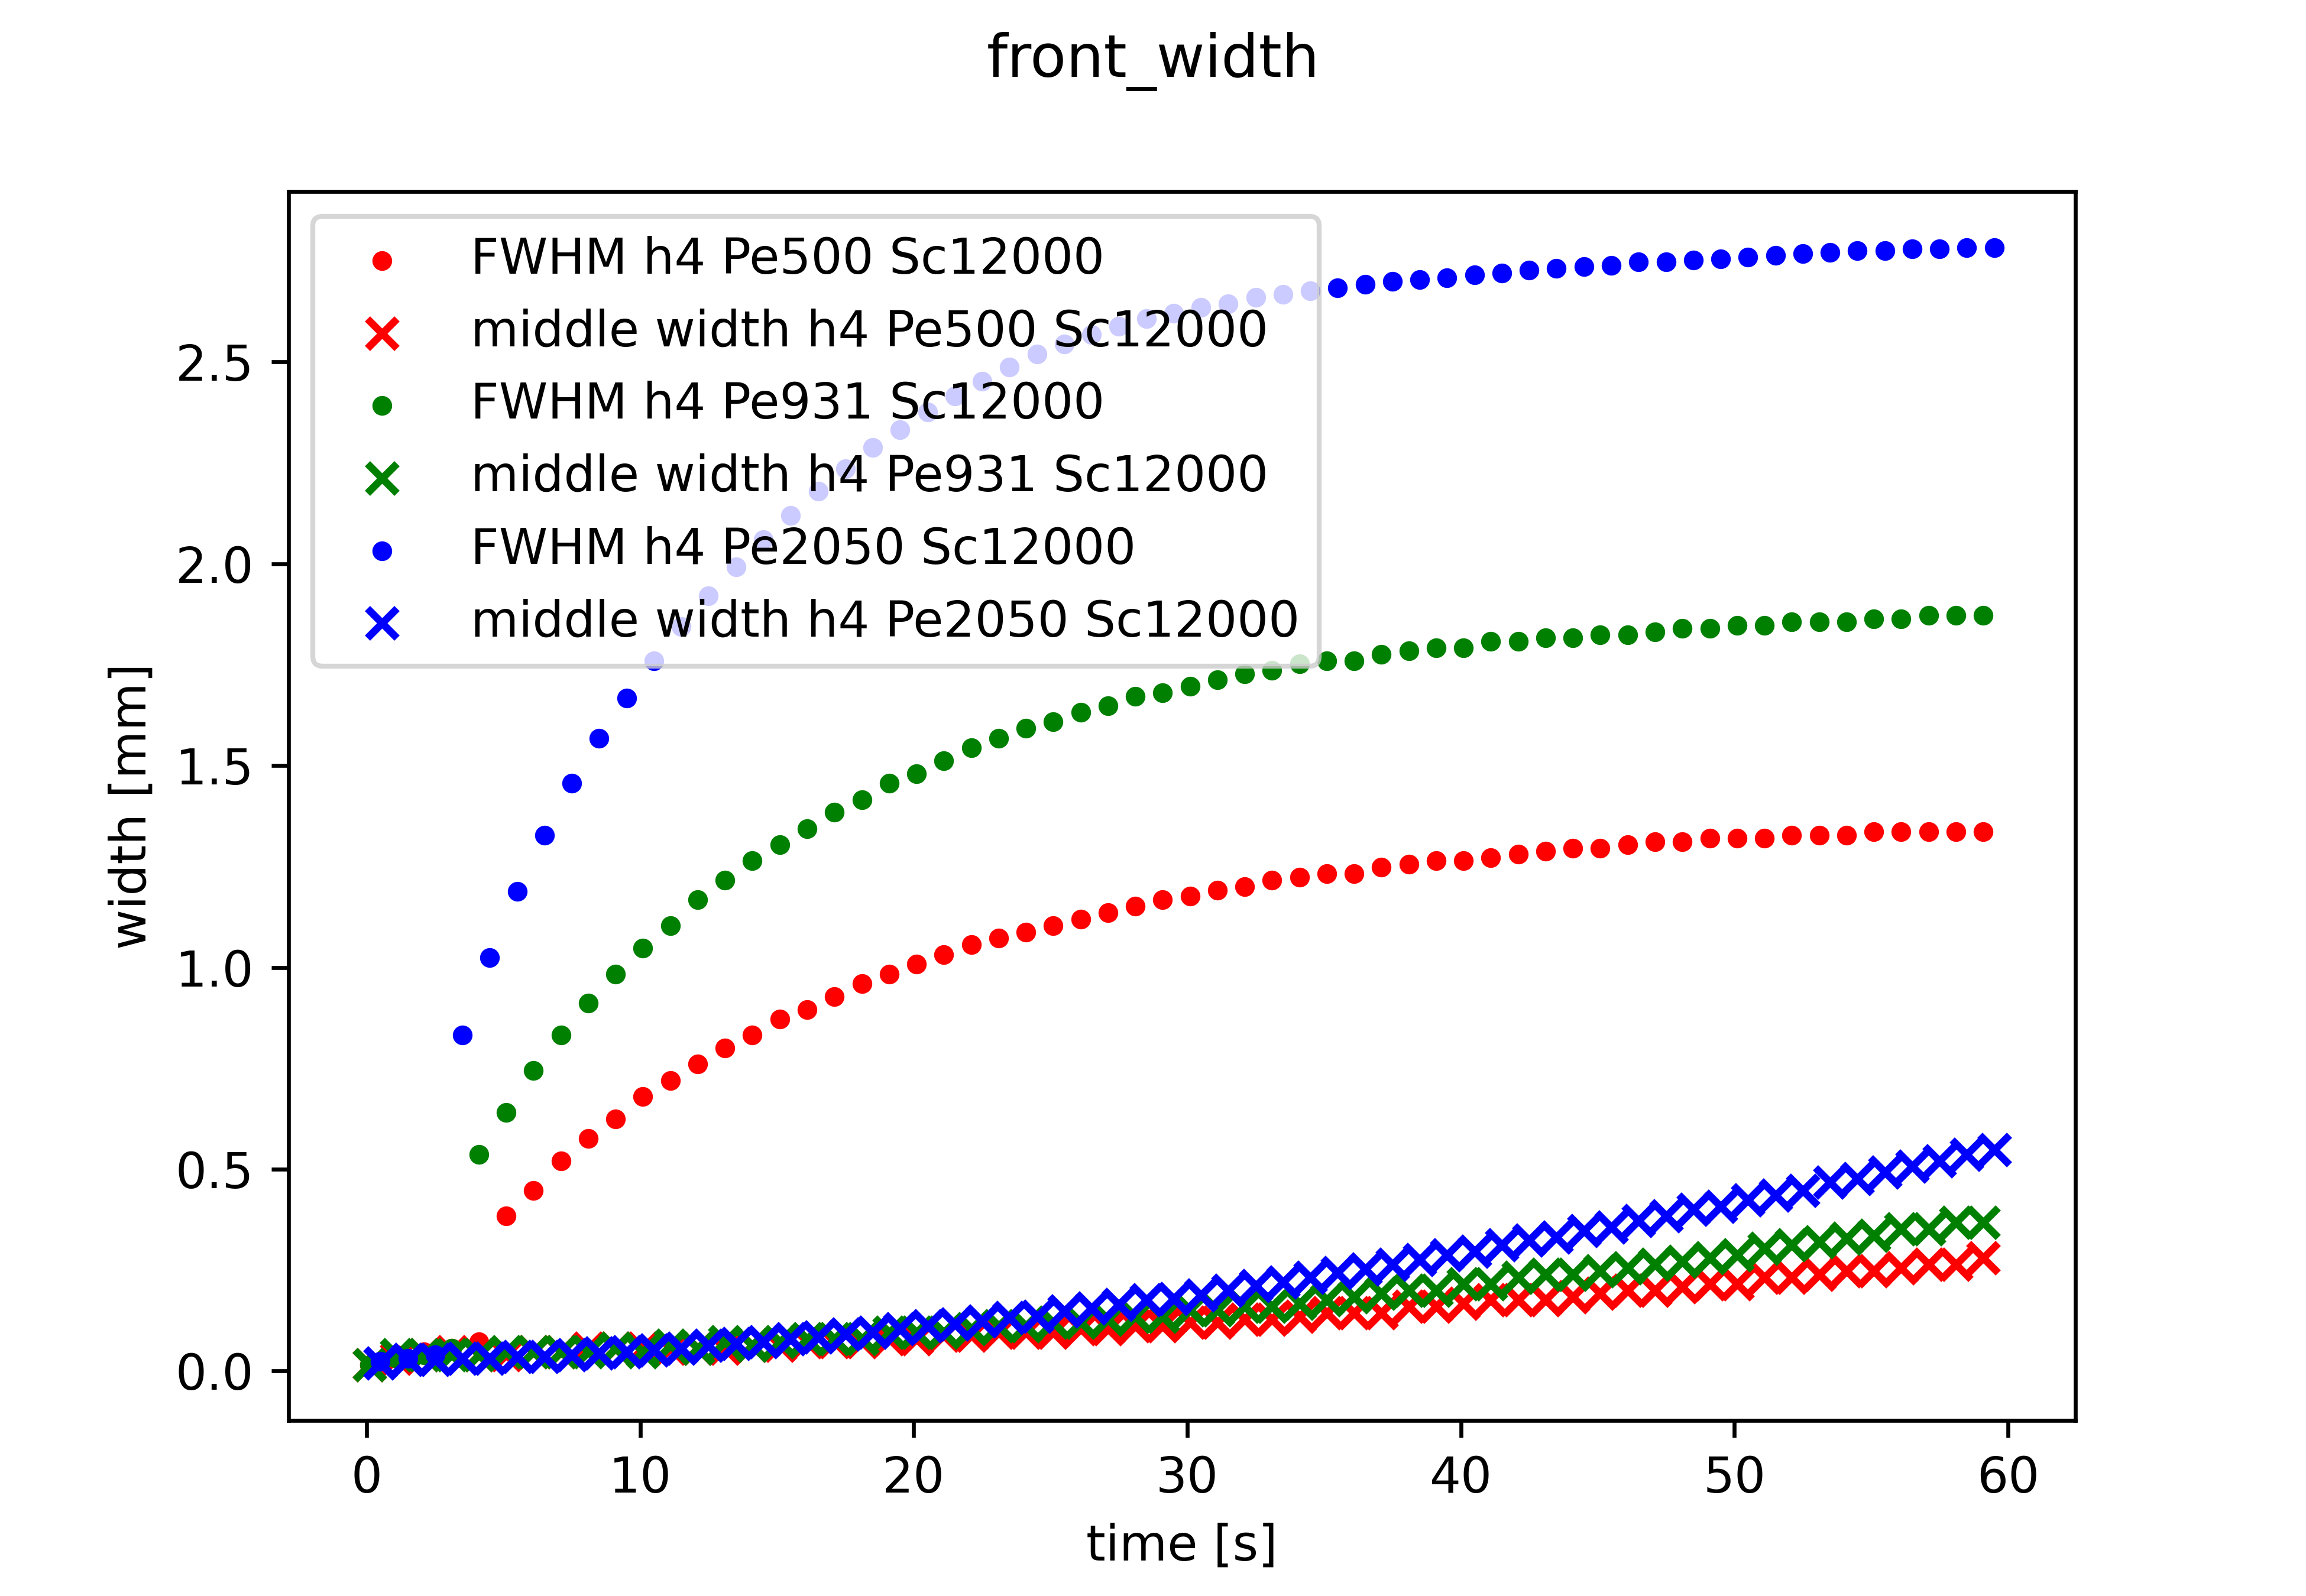
\includegraphics[width=.9\linewidth]{front_width_h4_SC12E4}
	\caption{front widths for h 0.4mm Sc 12000\label{fig: front_width_h4_SC12E4}}\bigskip
	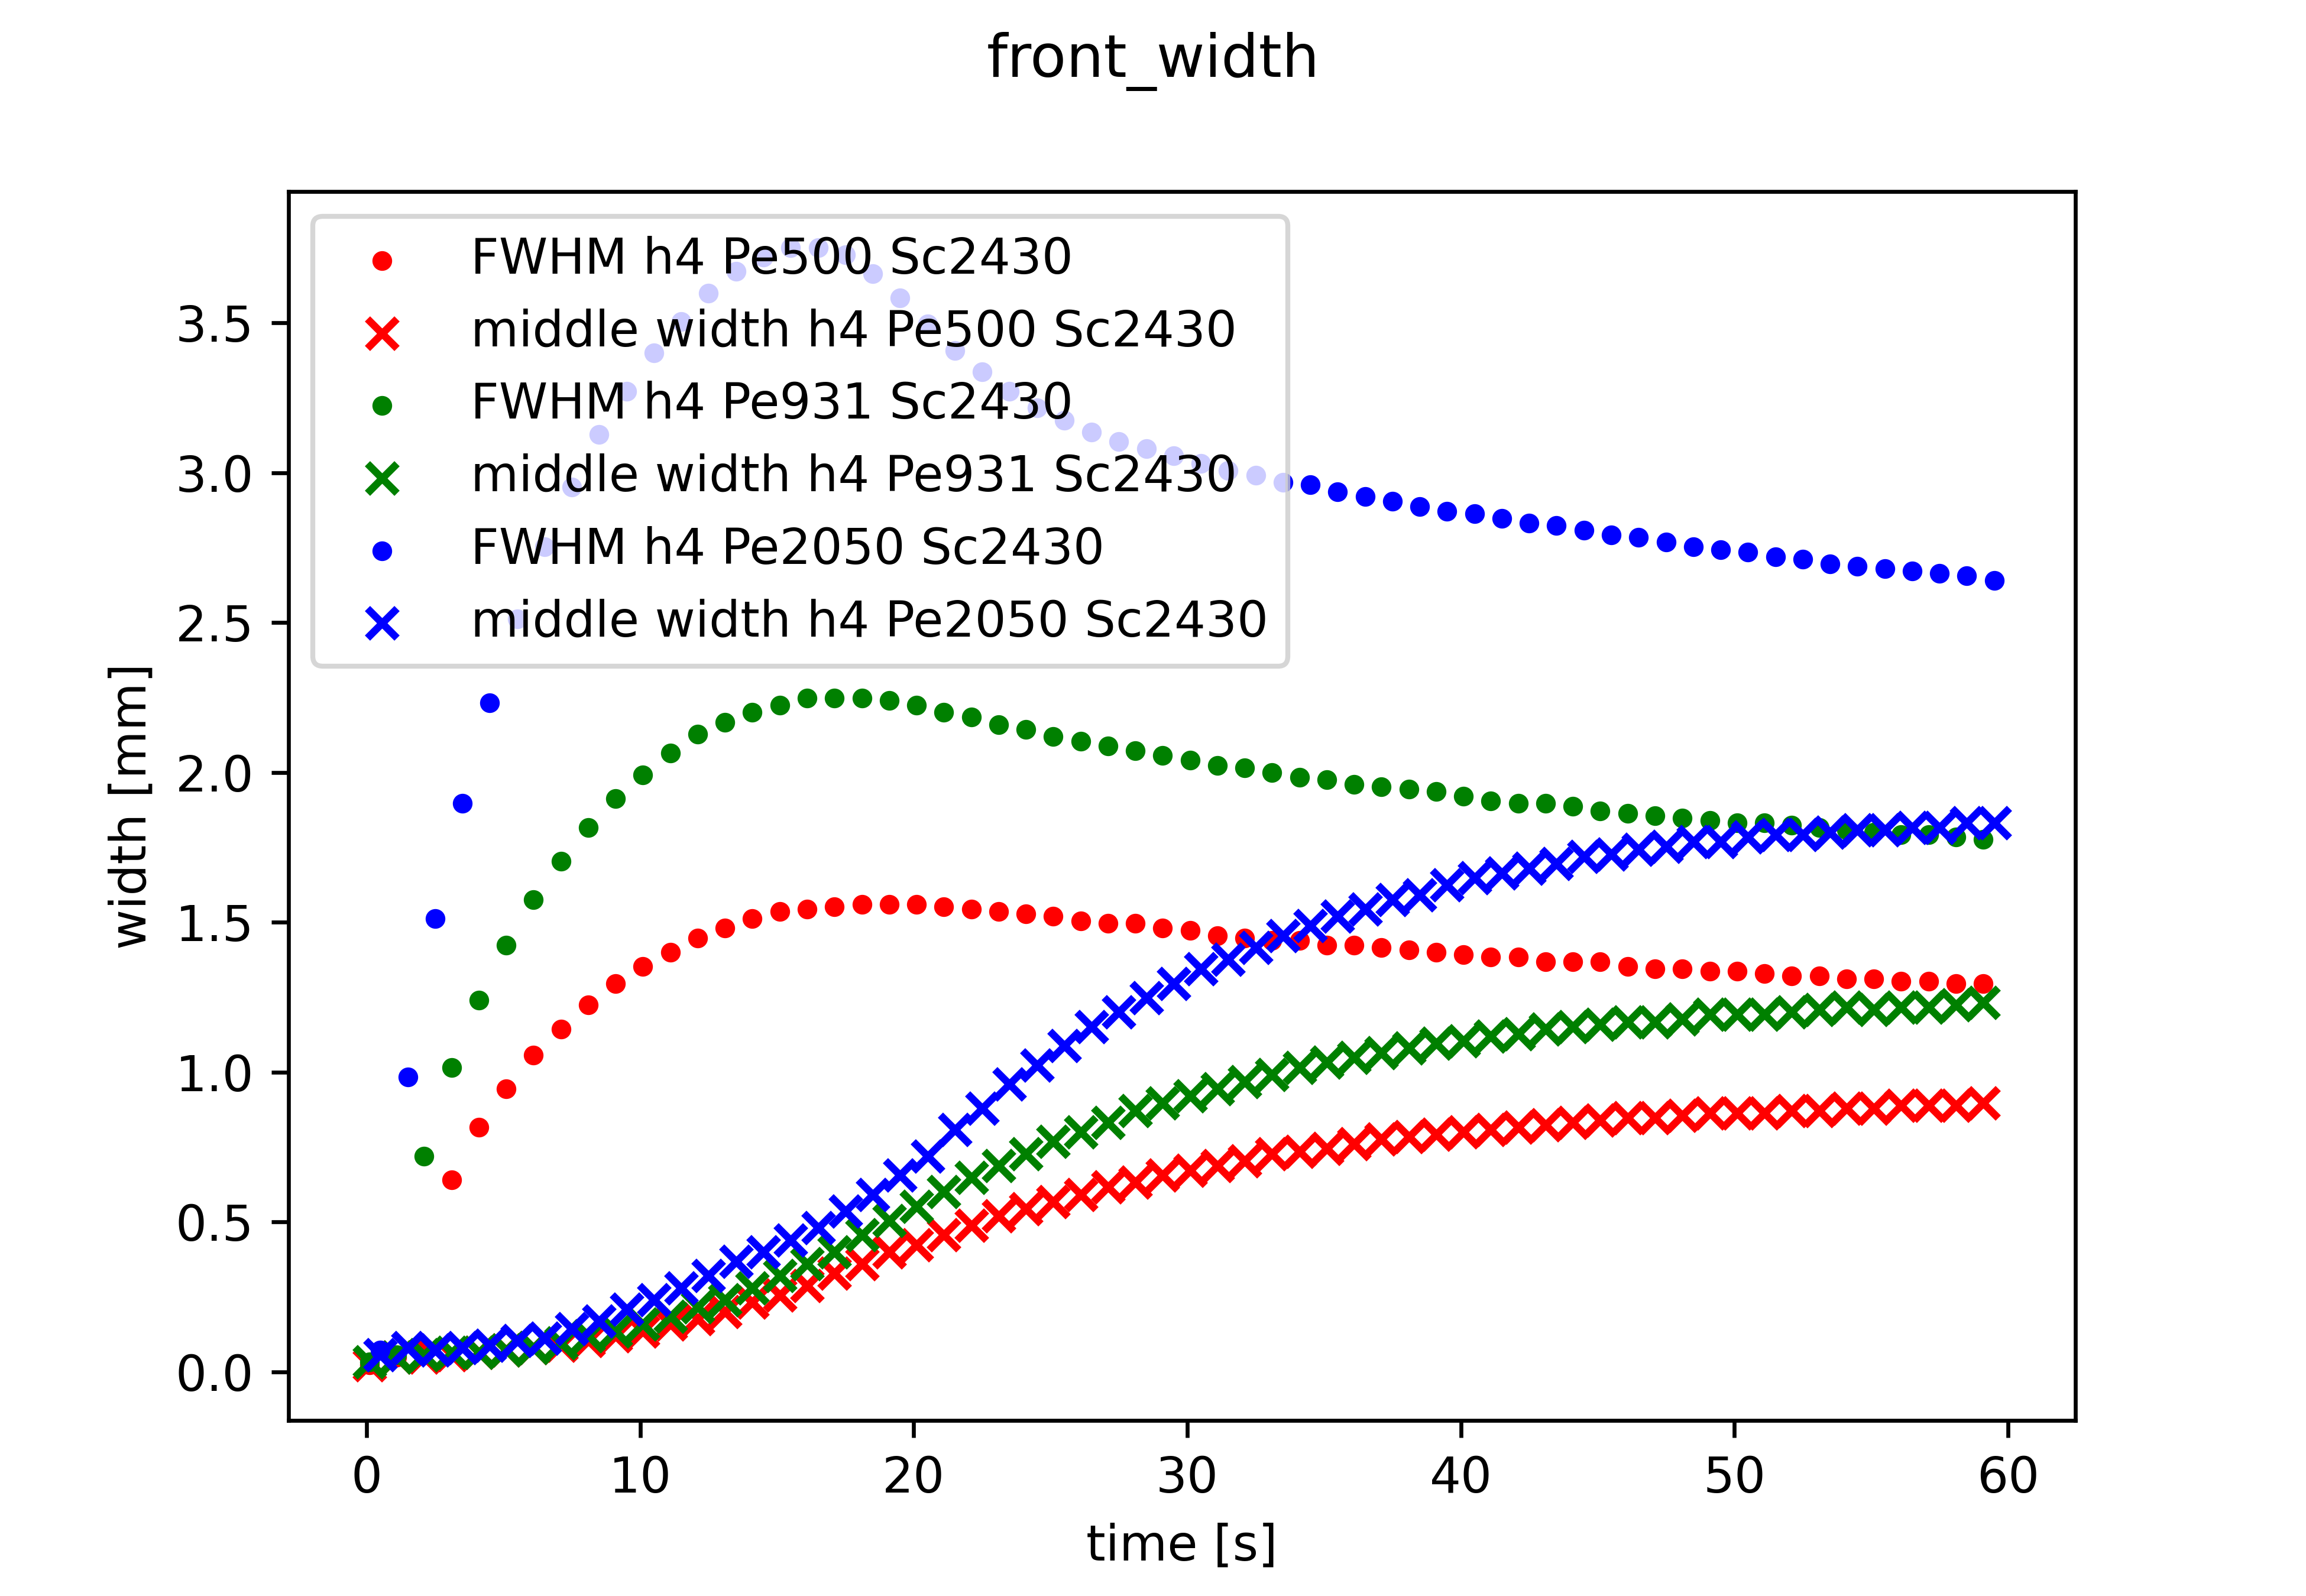
\includegraphics[width=.9\linewidth]{front_width_h4_SC243E3}
	\caption{front widths for h 0.4mm Sc 2430\label{fig: front_width_pos_h4_SC243E3}}
\end{figure}

\begin{figure}[htbp]
	\centering
	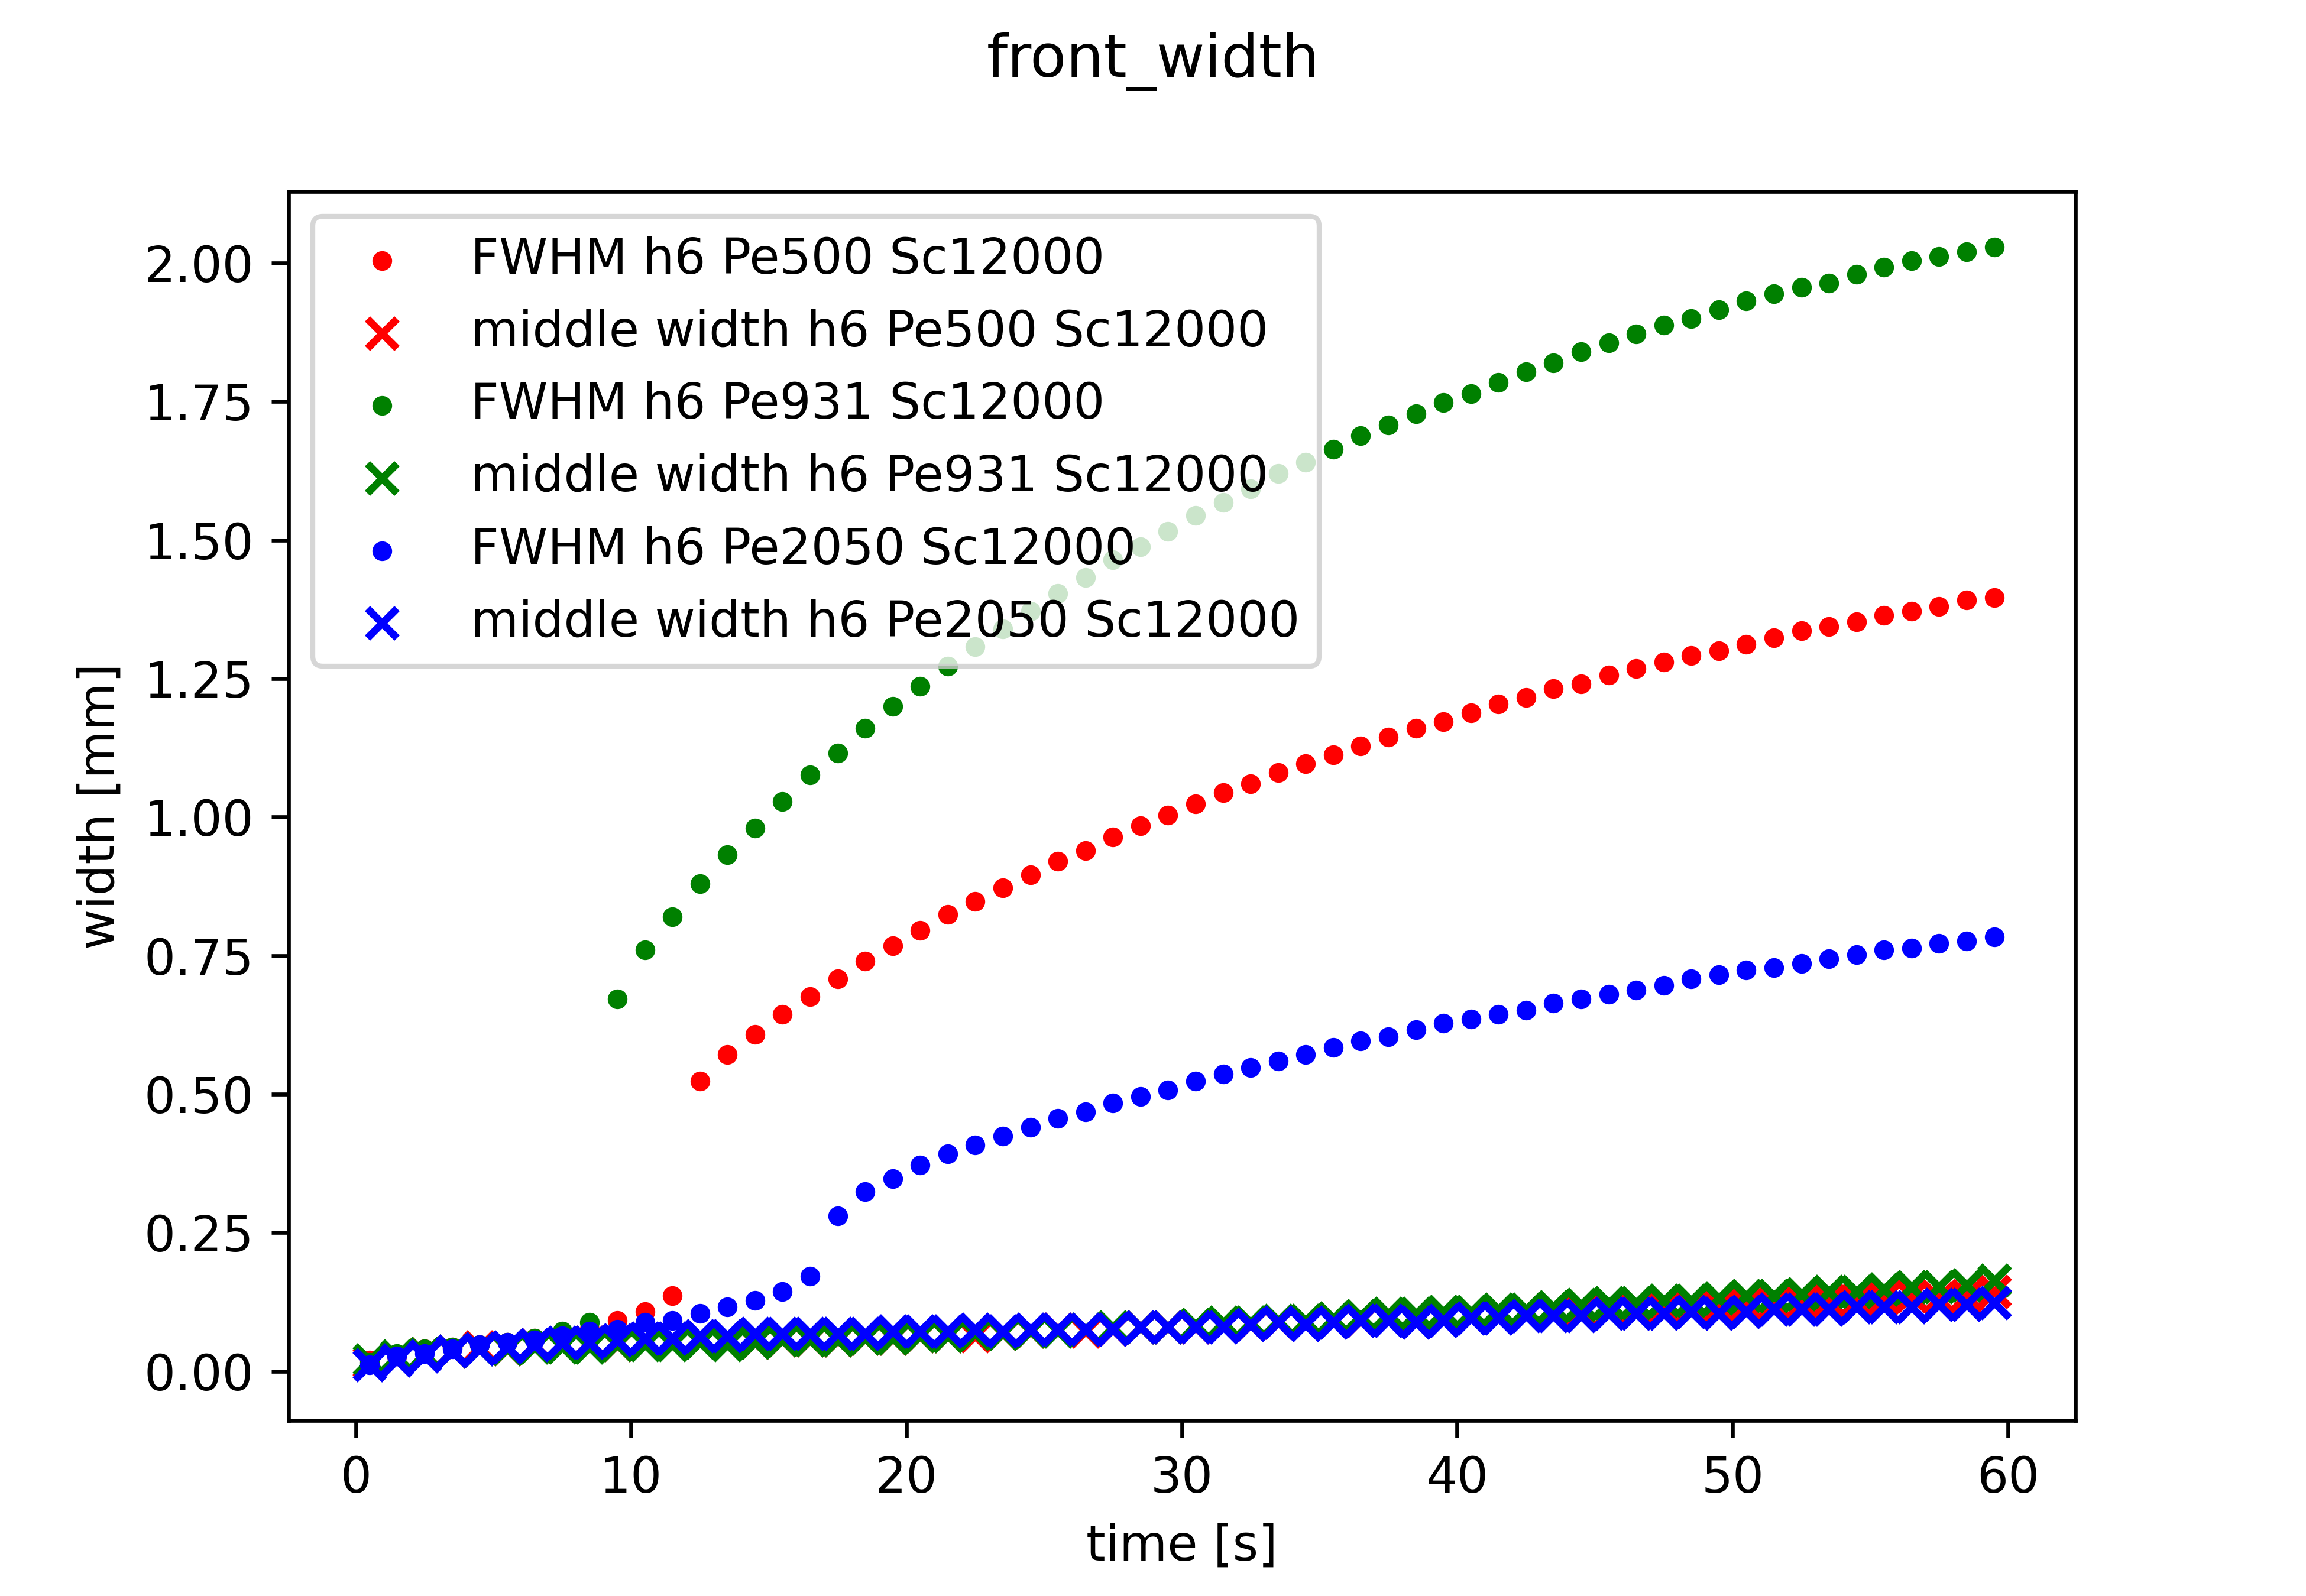
\includegraphics[width=.9\linewidth]{front_width_h6_SC12E4}
	\caption{front widths for h 0.6mm Sc 12000\label{fig: front_width_h6_SC12E4}}\bigskip
	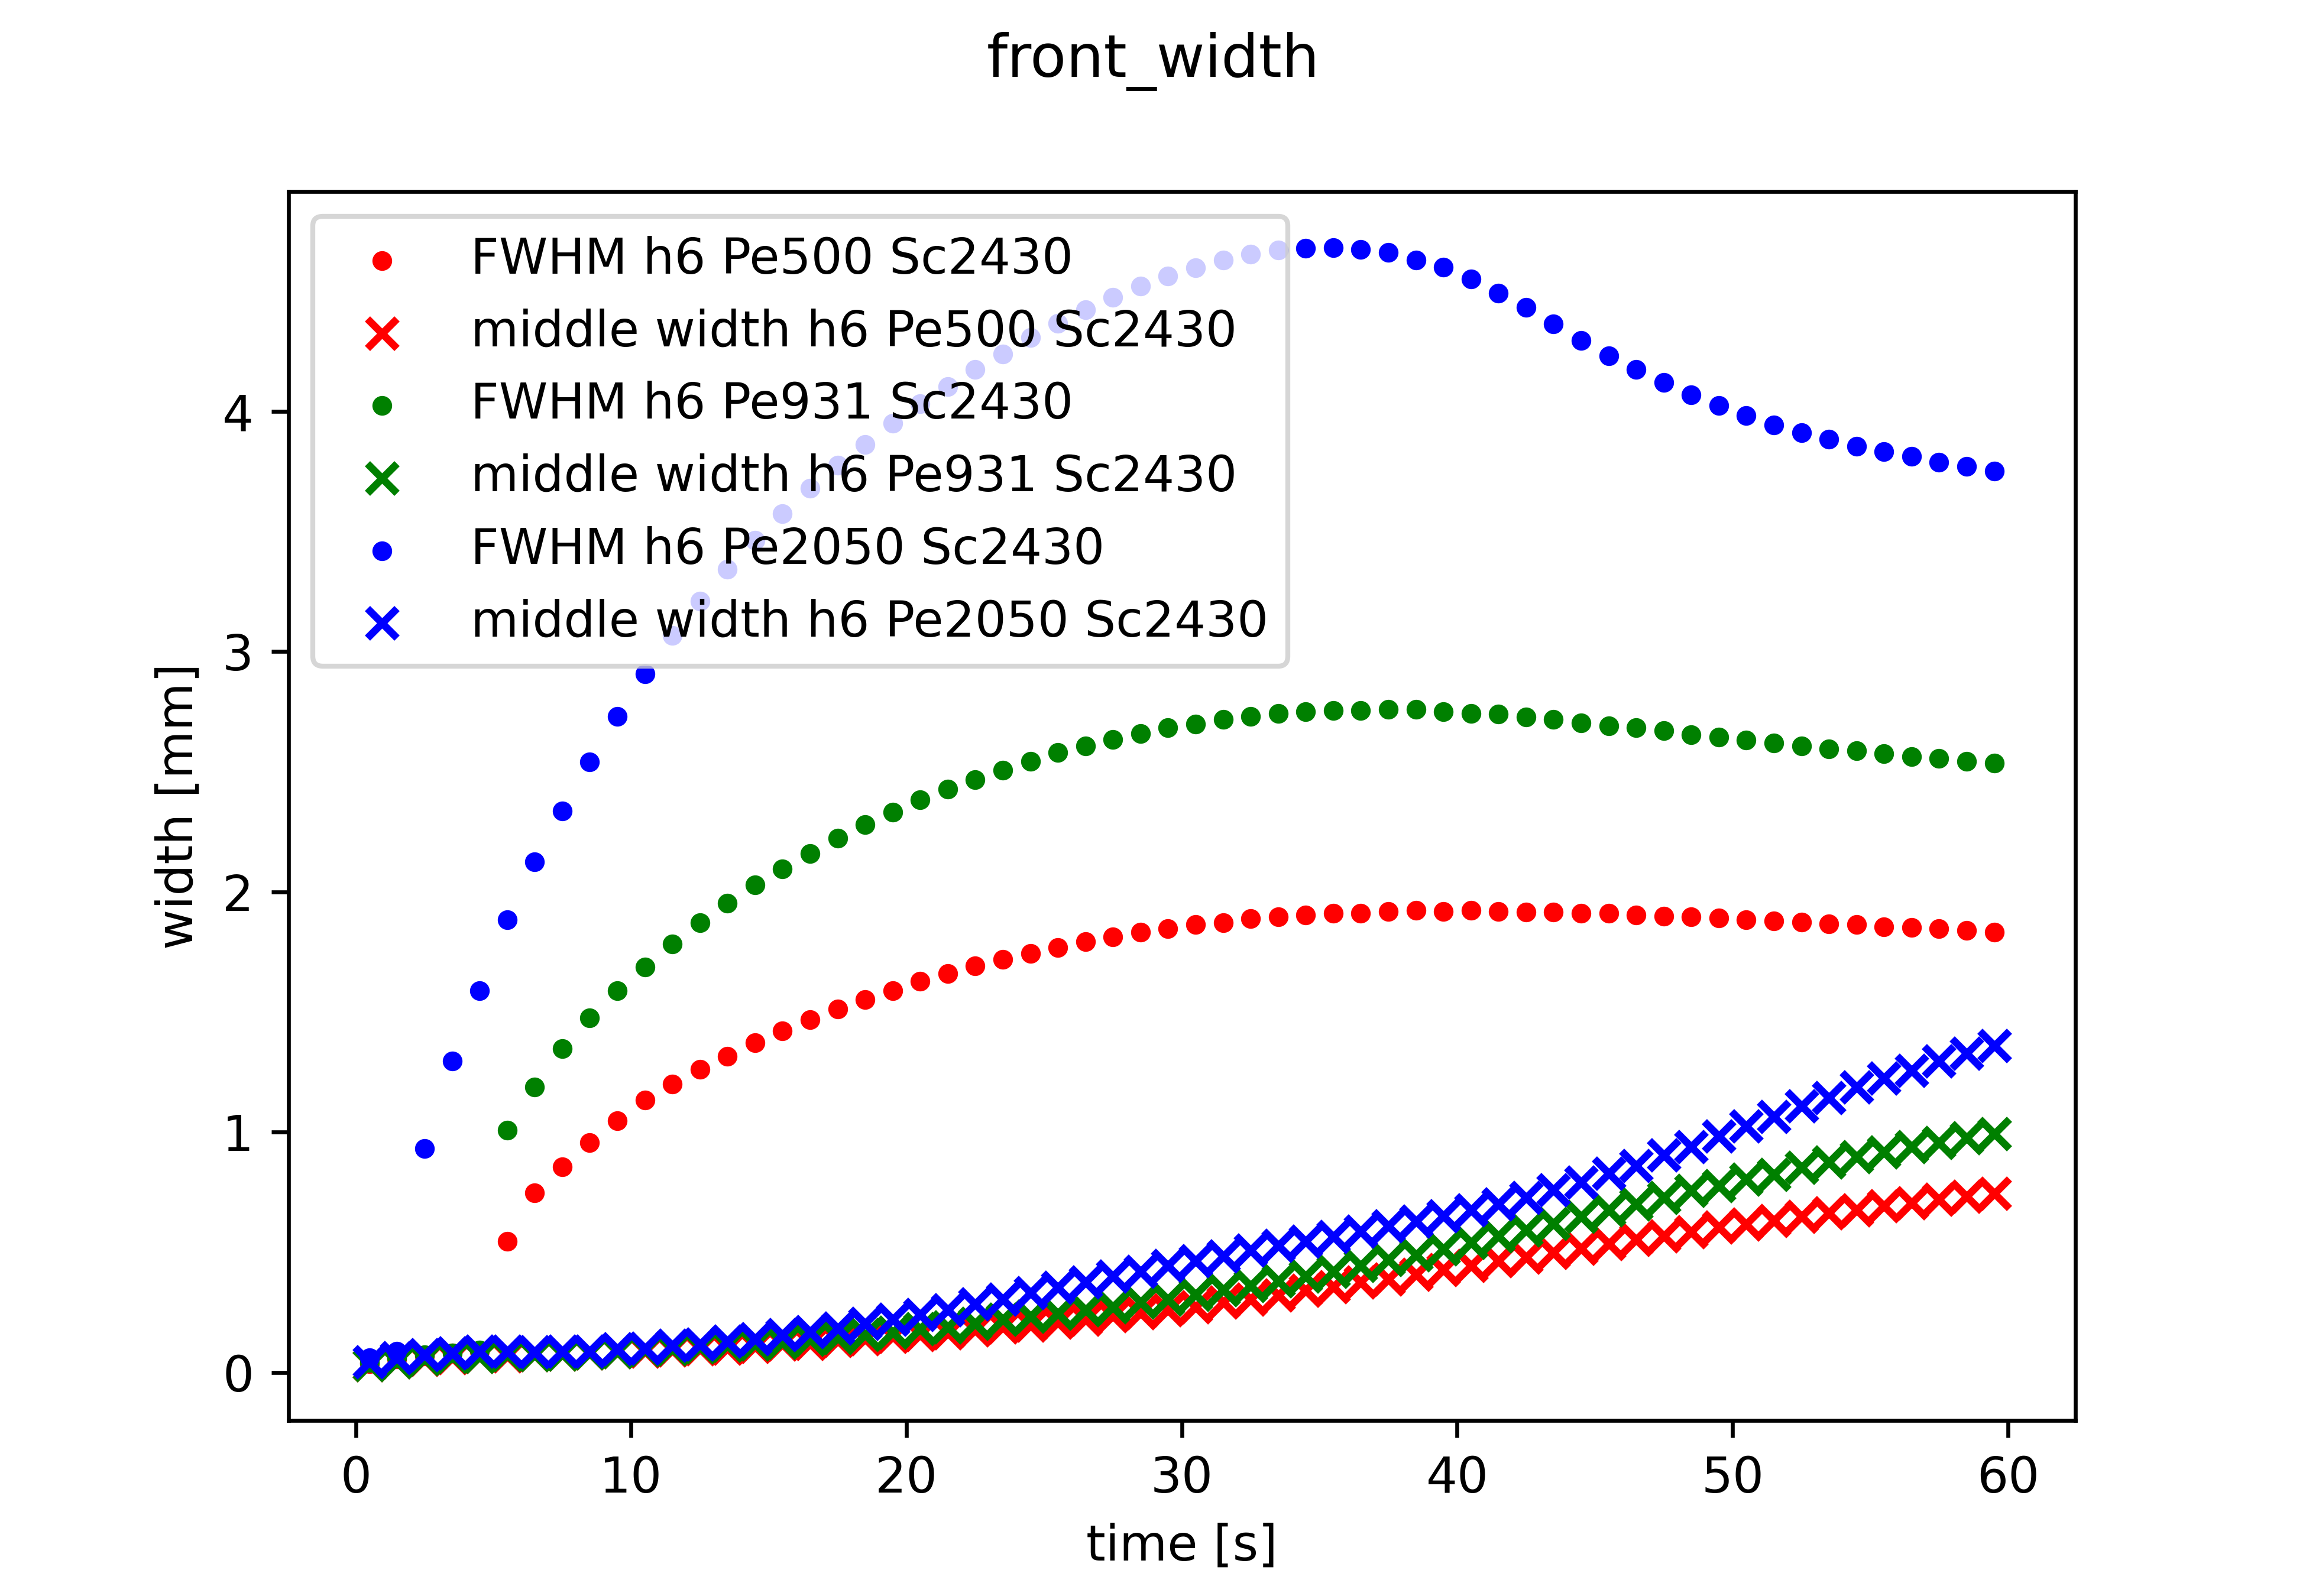
\includegraphics[width=.9\linewidth]{front_width_h6_SC243E3}
	\caption{front widths for h 0.6mm Sc 2430\label{fig: front_width_pos_h6_SC243E3}}
\end{figure}

\section{formed product}

\end{document}